\documentclass[a4paper, 12pt, fleqn, reqno, oneside]{report}
\usepackage[utf8]{inputenc}
\usepackage[T1]{fontenc}
\usepackage[utf8]{inputenc}
\usepackage{polski}
\usepackage[polish]{babel}
\usepackage{amsfonts}
\usepackage[hmargin=3.5cm, vmargin=3cm, hcentering]{geometry}
\usepackage{setspace} 
\usepackage{enumerate}
\usepackage{varwidth}
\usepackage{ulem}
\usepackage{xcolor}
\usepackage{url}
\usepackage{graphicx}
\usepackage{listings}
\usepackage[newfloat]{minted}
\usepackage{caption}
\usepackage{float}

\linespread{1.3}
\setlength{\parindent}{2em}

\usepackage[font=small,skip=1pt]{caption}
\newenvironment{code}{\captionsetup{type=listing}}{}
\SetupFloatingEnvironment{listing}{name=Załącznik}
\usepackage{sectsty, lmodern}
\setminted{baselinestretch=1.1}

\chapternumberfont{\fontsize{18pt}{0pt}\selectfont}
\chaptertitlefont{\fontsize{20pt}{0pt}\selectfont}
\sectionfont{\fontsize{14pt}{0pt}\selectfont}
%\linespread{1.25}


\lstdefinestyle{mystyle}{
    backgroundcolor=\color{backcolour},   
    commentstyle=\color{codegreen},
    keywordstyle=\color{magenta},
    numberstyle=\tiny\color{codegray},
    stringstyle=\color{codepurple},
    basicstyle=\ttfamily\footnotesize,
    breakatwhitespace=false,         
    breaklines=true,                 
    captionpos=b,                    
    keepspaces=true,                 
    numbers=left,                    
    numbersep=6pt,                  
    showspaces=false,                
    showstringspaces=false,
    showtabs=false,                  
    tabsize=2
}

\lstdefinelanguage{Dockerfile}
{
    morekeywords={
        FROM, RUN, CMD, LABEL, MAINTAINER, EXPOSE, ENV, ADD, COPY, ENTRYPOINT, VOLUME, USER, WORKDIR, ARG, ONBUILD, STOPSIGNAL, HEALTHCHECK, SHELL},
    morecomment=[l]{\#},
    morestring=[b]"
}

% https://www.overleaf.com/learn/latex/Code_Highlighting_with_minted
%RUBY
\definecolor{greyish}{rgb}{0.95,0.95,0.95}
\newmintedfile[scriptruby]{ruby}{
bgcolor=greyish,
fontfamily=tt,
linenos=true,
numberblanklines=true,
numbersep=2pt,
gobble=0,
frame=leftline,
framerule=0.2pt,
framesep=1mm,
funcnamehighlighting=true,
tabsize=4,
obeytabs=false,
mathescape=false
samepage=false,
showspaces=false,
showtabs =false,
texcl=false,
fontsize=\footnotesize,
breaklines=true
}

%BASH
\newmintedfile[scriptbash]{bash}{
bgcolor=greyish,
fontfamily=tt,
linenos=true,
numberblanklines=true,
numbersep=2pt,
gobble=0,
frame=leftline,
framerule=0.2pt,
framesep=1mm,
funcnamehighlighting=true,
tabsize=4,
obeytabs=false,
mathescape=false
samepage=false,
showspaces=false,
showtabs =false,
texcl=false,
fontsize=\footnotesize,
breaklines=true,
breakanywhere=true
}

\newmintedfile[scriptyaml]{yaml}{
bgcolor=greyish,
fontfamily=tt,
linenos=true,
numberblanklines=true,
numbersep=2pt,
gobble=0,
frame=leftline,
framerule=0.2pt,
framesep=1mm,
funcnamehighlighting=true,
tabsize=4,
obeytabs=false,
mathescape=false
samepage=false,
showspaces=false,
showtabs =false,
texcl=false,
fontsize=\footnotesize,
breaklines=true
}

\newmintedfile[scriptjs]{js}{
bgcolor=greyish,
fontfamily=tt,
linenos=true,
numberblanklines=true,
numbersep=2pt,
gobble=0,
frame=leftline,
framerule=0.2pt,
framesep=1mm,
funcnamehighlighting=true,
tabsize=4,
obeytabs=false,
mathescape=false
samepage=false,
showspaces=false,
showtabs =false,
texcl=false,
fontsize=\footnotesize,
breaklines=true
}

\newmintedfile[scriptjson]{js}{
bgcolor=greyish,
fontfamily=tt,
linenos=true,
numberblanklines=true,
numbersep=2pt,
gobble=0,
frame=leftline,
framerule=0.2pt,
framesep=1mm,
funcnamehighlighting=true,
tabsize=4,
obeytabs=false,
mathescape=false
samepage=false,
showspaces=false,
showtabs =false,
texcl=false,
fontsize=\footnotesize,
breaklines=true
}

\begin{document}

\begin{titlepage}
\vglue -15mm
\begin{figure}[h!]

\includegraphics{img/logous.png}
\end{figure}
\begin{flushright}
\vglue 1cm
{\Large Wydział Nauk Ścisłych i Technicznych}
\end{flushright}
\begin{center}
\vskip 2.5cm
{\Large\textbf{Ewa Namysł}}
\vskip 0.5cm
{\Large Numer albumu 292001}
\vfill
\begin{doublespace}
{\huge \bf Wdrożenie i testowanie środowiska klastrowego w oparciu o oprogramowanie Kubernetes}
\end{doublespace}
\vfill
{\large PRACA DYPLOMOWA\\INŻYNIERSKA}
\end{center}
\vskip 2.5cm
\begin{flushright}
\parbox{4.5cm}\Large\textbf{{Imię i nazwisko promotora\\
dr hab. prof UŚ Seweryn Kowalski
}}
\end{flushright}
\vspace{2.5cm}
\begin{center}
\Large Katowice 2023
\end{center}
\end{titlepage}




\iffalse
    \begin{titlepage}
    \begin{center}
    {\Large Uniwersytet Śląski w Katowicach}
    \vskip 0.7cm
    {\Large  Wydział Nauk Ścisłych i Technicznych}
    \vskip 2.5cm
    {\Large \bf Ewa Namysł}
    \vskip 1cm
    {\large Numer albumu 292001}
    \vskip 2.5cm
    \begin{doublespace}
    {\huge \bf Wdrożenie i testowanie środowiska klastrowego w oparciu o oprogramowanie Kubernetes}
    \end{doublespace}
    \vskip 2.5cm
    {\large PRACA DYPLOMOWA\\INŻYNIERSKA}
    \end{center}
    \vspace{3.5cm}
    \begin{flushright}
    \parbox{6.5cm}{Promotor: \\
    dr hab. Seweryn Kowalski}
    \end{flushright}
    \vspace{1.5cm}
    \begin{center}
    Katowice 2023
    \end{center}
    
    \newpage
    \thispagestyle{empty}
    \begin{small}
    \noindent
    Słowa kluczowe: Docker, Kubernetes, Linux, wirtualizacja\\
    
    \textbf{Oświadczenie autora pracy}\\[0.5cm]
    Ja niżej podpisana:\\
    
    
    {\raggedright imię} i nazwisko: Ewa Namysł\\
    autor pracy dyplomowej pt.: Docker i Kubernetes w zarządzaniu projektem informatycznym\\
    numer albumu: 292001\\
    studentka Wydziału Nauk Ścisłych i Technicznych Uniwersytetu Śląskiego w Katowicach, kierunku studiów: informatyka stosowana\\
    
    \noindent Oświadczam, że ww. praca dyplomowa:
    \begin{itemize}
    \item została przygotowana przeze mnie samodzielnie\footnote{\scriptsize uwzględniając merytoryczny wkład promotora (w ramach prowadzonego seminarium dyplomowego)},
    \item nie narusza praw autorskich w rozumieniu ustawy z dnia 4 lutego 1994 r. o prawie autorskim i prawach pokrewnych (tekst jednolity Dz. U. z 2006 r. Nr 90, poz. 631, z późn. zm.) oraz dóbr osobistych chronionych prawem cywilnym,
    \item nie zawiera danych i informacji, które uzyskałam w sposób niedozwolony,
    \item nie była podstawą nadania dyplomu uczelni wyższej lub tytułu zawodowego ani mnie, ani innej osobie.
    \end{itemize}
    \vskip 0.5cm
    Oświadczam również, że treść pracy dyplomowej zamieszczonej przeze mnie w Archiwum Prac Dyplomowych jest identyczna z treścią zawartą w wydrukowanej wersji pracy.\\[0.5cm]
    \textbf{Jestem świadoma odpowiedzialności karnej za złożenie fałszywego oświadczenia.}\\[1cm]
    
    \footnotesize{\parbox{4cm}{\dotfill\center{\footnotesize Data}}\hfill\parbox{5cm}{\dotfill\center{\footnotesize Podpis autora pracy}}}
    \end{small}
    \end{titlepage}
\fi


\setcounter{page}{1}
\tableofcontents 

\chapter*{Wstęp}
\addcontentsline{toc}{chapter}{Wstęp}

W przeciągu kilku ostatnich lat Kubernetes stał się jednym z najbardziej popularnych wolnoźródłowych rozwiązań zarządzania infrastrukturą w projektach informatycznych. Wykorzystanie tej platformy usprawnia proces szybkiego dostarczania skonteneryzowanych aplikacji, a ponadto ułatwia i automatyzuje część zadań związanych z ich administracją. 

W niniejszej pracy stworzono dwa rodzaje klastrów Kubernetesa oraz przeprowadzono testy, służące oszacowaniu ich wydajności. W tym celu wykorzystano narzędzia z otwartym źródłem, które umożliwiają konteneryzację aplikacji, automatyzację powtarzalnych zadań, monitoring oraz testowanie stworzonej infrastruktury. Ponadto opisano teoretyczne aspekty związane z wirtualizacją, konteneryzacją oraz orkiestracją kontenerami. 


\chapter{Wirtualizacja}

Jednym z zastosowań wirtualizacji jest jednoczesne uruchomienie wielu instancji systemu operacyjnego na tym samym sprzęcie fizycznym. Oprogramowanie wirtualizacyjne rozdziela zasoby procesora, pamięci oraz operacje wejścia-wyjścia, przydzielając je odseparowanym od siebie wirtualnym maszynom \cite{biblia_linux}.

Wirtualizacja rozwijana jest od lat 60. XX wieku. Na początku opracowywana była przez firmę IBM z myślą o wyspecjalizowanych mainframe'ach. W tamtym okresie technologia ta nie zyskała jednak popularności. Było to spowodowane głównie ograniczeniami technologicznymi i częściej wykorzystywanym \textit{time-sharingiem}, który pozwalał wielu użytkownikom wykonywać operacje na jednej maszynie w tym samym czasie \cite{idkrtm, arundel}. 

Przełom nastąpił wraz ze wzrostem roli infrastruktury informatycznej w biznesie. Jednym z największych ówczesnych problemów był transfer oprogramowania na nowy sprzęt. Było to zwykle niemożliwe bez wprowadzenia zmian w samym oprogramowaniu lub odtworzeniu go na architekturę nowej maszyny. To z kolei generowało koszty i wymagało czasu. 

Kolejną trudnością był sposób przechowywania aplikacji na serwerach. Jednoczesne uruchamianie wielu aplikacji na pojedynczym fizycznym serwerze nierzadko stwarzało problemy, tj. gdy jedna z aplikacji zaczynała zużywać więcej zasobów, spowalniana była praca pozostałych. W efekcie każda aplikacja umieszczana była na osobnym, dedykowanym jej serwerze \cite{ibm, kubernetes}. Pojedyncza aplikacja przez większość czasu nie wykorzystywała jednak pełnej mocy obliczeniowej serwera, co znacznie wpłynęło na zwiększenie kosztów sprzętu oraz jego utrzymania, lecz dostępne już zasoby nadal pozostawały niewykorzystane w optymalny sposób. Ww. czynniki oraz postęp technologiczny lat 90. wpłynęły na gwałtowny rozwój wirtualizacji.

\section{Hipernadzorca}
Instancje maszyn wirtualnych (ang. \textit{virtual machine}, VM) są zarówno tworzone, jak i kontrolowane przez tzw. hipernadzorcę (ang. \textit{hypervisor}). Hipernadzorca stanowi także warstwę izolującą zasoby hosta od wirtualnych maszyn oraz przydziela im wspomniane zasoby. Wyróżniane są dwa rodzaje hipernadzorców:

\begin{enumerate}[(1)]
    \item {\itshape natywny} lub {\itshape bare metal}, działający bezpośrednio na warstwie sprzętowej komputera-gospodarza i zastępujący tym samym system operacyjny, 
    
    \item {\itshape hostowany}, uruchamiany jako program na komputerze-gospodarzu \cite{biblia_linux}.
\end{enumerate}

Pierwszy z nich najczęściej wykorzystywany jest w rozwiązaniach chmurowych i centrach danych, gdzie wymagana jest szybkość i bezpieczeństwo. Hipernadzorca typu drugiego (Rysunek 1.1) stanowi z kolei dodatkową warstwę pomiędzy systemem operacyjnym hosta a wirtualnymi maszynami.

\begin{figure}[h]
    \centering
    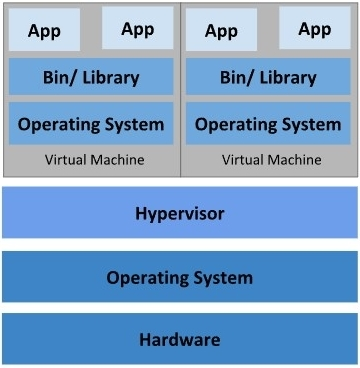
\includegraphics[width=0.6\textwidth]{img/rozdzial1-1.jpg}
    \caption{Wirtualizacja z hipernadzorcą typu drugiego \cite{kubernetes}}
\end{figure}
\newpage

\section{Zastosowania maszyn wirtualnych}
Spośród najpopularniejszych zastosowań maszyn wirtualnych można wyróżnić:
\begin{enumerate}[(1)]
    \item użytkowanie aplikacji lub programów natywnie stworzonych dla konkretnego systemu operacyjnego lub niekompatybilnych z aktualnym systemem,
    \item izolowanie oprogramowania lub wykonywanie zadań potencjalnie niebezpiecznych dla komputera-gospodarza,
    \item testowanie oprogramowania w środowiskach różnych systemów operacyjnych,
    \item przetwarzanie w chmurze \cite{ibm}. 
\end{enumerate}

\section{Zalety i wady wirtualizacji}
Dzięki wirtualizacji możliwe jest efektywne wykorzystywanie zasobów sprzętowych, co przekłada się na niższe koszty eksploatacji hardware'u. Aplikacje w zwirtualizowanym środowisku są odizolowane od siebie i nie mają dostępu do danych przechowywanych na innych wirtualnych maszynach  (Rysunek 1.1), a każda z maszyn ma swój własny system operacyjny, system plików, biblioteki itd. Ponadto aplikacje niekompatybilne z nowszymi wersjami systemu można z powodzeniem uruchamiać w wirtualnych środowiskach. 

Pomimo zmniejszenia ilości sprzętu fizycznego i relatywnie krótkiego czasu, którego potrzebujemy do odtworzenia środowiska, nadal konieczne jest aktualizowanie i utrzymywanie systemów operacyjnych na wirtualnych maszynach. Co więcej, w przypadku problemów sprzętowych dostęp do wszystkich maszyn wirtualnych na danym hoście może być niemożliwy. System operacyjny zajmuje również część pamięci wydzielonej dla konkretnej wirtualnej maszyny, więc jeśli systemy operacyjne dublują się, powstaje problem redundancji, tj. znaczna część miejsca zajmowana jest przez te same systemy \cite{ibm}. 
\newpage

\section{Wykorzystane technologie}
Poniżej krótkie omówienie wykorzystywanych w pracy technologii z otwartym źródłem, umożliwiających wirtualizację w systemach operacyjnych opartych na jądrze Linuxa:
\begin{itemize}
    \item KVM (ang. \textit{Kernel-based Virtual Machine}) \cite{kvm} jest środowiskiem wirtualizacyjnym, wbudowanym bezpośrednio w jądro Linuxa. Funkcję hipernadzorcy pełni samo jądro, a uruchamiane maszyny wirtualne są zwykłymi procesami. 
    
    \item QEMU (\textit{Quick Emulator}) \cite{qemu} to emulator maszyn, który wykorzystywany jest również w roli hipernadzorcy typu drugiego. QEMU zintegrowany z KVM oferuje emulację sprzętową, pozwalając równocześnie na wykonywanie zadań maszyny wirtualnej bezpośrednio na procesorze komputera-gospodarza, osiągając szybkość zbliżoną do maszyn fizycznych. 

    \item Biblioteka \textit{libvirt} \cite{libvirt} składa się z API (ang. \textit{application programming interface}), daemona oraz narzędzi wiersza poleceń. Głównym celem biblioteki jest uproszczenie i ujednolicenie procesu zarządzania maszynami wirtualnymi z różnymi hipernadzorcami. Dzięki wspomnianej bibliotece ułatwiona jest konfiguracja maszyn bazujących na wirtualizacji KVM/QEMU.

    \item Vagrant \cite{vagrant} to otwartoźródłowe oprogramowanie służące do szybkiego tworzenia i konfigurowania maszyn wirtualnych. Do działania niezbędny jest hipernadzorca - najszerzej wspierany przez oprogramowanie jest VirtualBox, jednak udostępniane są również rozszerzenia dla innych platform, w tym \textit{libvirt}. Definiowanie parametrów i budowanie maszyn oparte jest na pliku konfiguracyjnym \textit{Vagrantfile}, w którym umieszczane są informacje o środowisku. Podawany jest konkretny system operacyjny, pakiety i biblioteki do zainstalowania, konfiguracja sieci itp. Dzięki wykorzystaniu plików maszyna o tych samych parametrach może być wielokrotnie tworzona w prosty sposób od nowa. Ponadto Vagrant umożliwia automatyzację, m.in. za pomocą skryptów powłoki czy też Ansible.
\end{itemize}



%%%%%%%%%%%%%%%%%%%%%%%%%%%%%%%%%%%%%%%%%%


\chapter{Konteneryzacja}

Konteneryzacja jest procesem polegającym na spakowaniu aplikacji wraz z niezbędnymi bibliotekami oraz innymi zależnościami do tzw. kontenera (ang. \textit{container}) \cite{biblia_linux}. Kontenery budowane są na podstawie obrazów (ang. \textit{image}) - plików tekstowych, w których definiowana jest pełna konfiguracja.

Kontenery są bardzo lekkie i przenośne, ponieważ nie zawierają pełnego systemu operacyjnego, lecz korzystają z funkcji systemowych komputera-gospodarza (Rysunek 2.1). 

\begin{figure}[h]
    \centering
    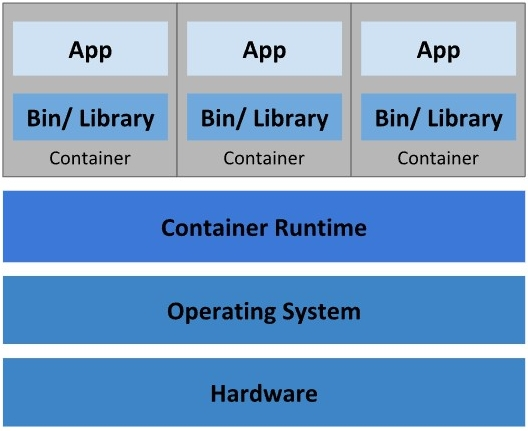
\includegraphics[width=0.6\textwidth]{img/rozdzial1-2.jpg}
    \caption{Konteneryzacja \cite{kubernetes}}
\end{figure}

Pierwszym rozwiązaniem, przypominającym w założeniu współczesne kontenery, była wprowadzona w 2000 roku komenda systemu FreeBSD 4.X \textit{jail} \cite{freebsd, nickoloff}. Umożliwiała ona izolowanie m.in. procesów, sieci, użytkowników i systemów plików. Polecenie miało jednak ograniczenia w zakresie bezpieczeństwa. 

Pięć lat później Google rozpoczęło pracę nad \textit{cgroups}. Mechanizm ten pozwalał nie tylko izolować procesy, ale też ograniczyć zużycie zasobów i wkrótce stał się integralną częścią jądra Linuxa \cite{nickoloff}. 
Od tego momentu rozwijany był również projekt Linux Containers (skrótowo LXC) \cite{lxc}, który miał na celu tworzenie skonteneryzowanych instancji pełnoprawnych systemów linuxowych pozbawionych własnego jądra, a działających bezpośrednio na jądrze systemu-gospodarza. Dzięki temu wewnątrz kontenerów LXC może działać równolegle wiele procesów.

W 2013 roku upublicznione zostało oprogramowanie Docker o otwartym źródle \cite{docker}. Docker, choć korzysta m.in. z \textit{cgroups} oraz rozwiązań LXC, powstał z myślą o tworzeniu kontenerów z tylko jedną aplikacją i ograniczonymi funkcjonalnościami systemu. Obecnie pozostaje najczęściej wykorzystywaną technologią tworzenia kontenerów.

\section{Docker}

Platforma Docker posiada rozbudowany zestaw poleceń, dzięki którym możliwe jest szybkie budowanie, modyfikowanie oraz niszczenie kontenerów. Bardziej optymalną metodą jest jednak tworzenie obrazów poprzez plik tekstowy \textit{Dockerfile}. W pliku tym zawierane są komendy oraz instrukcje dotyczące procesu budowania i konfiguracji. Dzięki temu proces jest zautomatyzowany, a kontener o tej samej specyfikacji może być utworzony ponownie. 

Docker posiada również zestaw dodatkowych funkcjonalności, ułatwiających przechowywanie danych czy też pracę nad złożonymi aplikacjami zbudowanymi z wielu kontenerów. 

Ponadto Docker współtworzy publiczne repozytorium Docker Hub \cite{dockerhub}, gdzie użytkownicy oraz firmy mogą udostępniać stworzone przez siebie obrazy. Tego typu predefiniowane obrazy mogą być pobierane i wykorzystywane w celu dalszej modyfikacji.

\section{Kontenery Dockera a wirtualizacja}

Kontenery Dockera nie wykorzystują wirtualizacji sprzętowej \cite{nickoloff}, która jest kluczowa dla działania maszyn wirtualnych. Wewnątrz znajduje się tylko aplikacja, niezbędne biblioteki oraz ograniczone funkcjonalności systemowe. Uruchomione w kontenerze programy komunikują się bezpośrednio z jądrem systemowym komputera-gospodarza. Brak pełnego systemu operacyjnego sprawia, że kontenery uruchamiane są znacznie szybciej od maszyn wirtualnych \cite{krochmalski}.
 
Kontenery nie są związane z leżącymi poniżej warstwami infrastruktury ani nie są zarządzane przez hipernadzorcę, więc mogą być w niezwykle prosty sposób przenoszone pomiędzy różnymi maszynami lub dostarczycielami rozwiązań chmurowych \cite{poulton}. Umożliwia to przyspieszenie procesu udostępniania, budowania i wdrażania kolejnych wersji oprogramowania.

Nie oznacza to jednak, że wybór jednej z tych technologii ogranicza możliwość użycia drugiej. Obecnie najczęściej spotykane są rozwiązania łączące zarówno wirtualizację, jak i konteneryzację \cite{nickoloff}.

\section{Korzyści i ograniczenia Dockera}

Spośród zalet Dockera można wymienić:

\begin{enumerate}[(1)]
    \item szybkość w tworzeniu, niszczeniu i modyfikowaniu kontenerów,
    \item przenośność, która pozwala na uruchamianie aplikacji na różnych maszynach, 
    \item raz stworzony kontener działa wszędzie tak samo i nie wymaga instalowania dodatkowych paczek po stronie \textit{hosta} - brak konflików związanych z instalacją różnych wersji bibliotek itd.,
    \item niezmienność obrazów - plik \textit{Dockerfile} zapewnia instrukcję instalacyjną do tworzenia kolejnych instancji, 
    \item izolacja aplikacji od siebie, jak i od systemu operacyjnego \cite{nickoloff, krochmalski}.
\end{enumerate}

Należy jednak brać pod uwagę również ograniczenia tej technologii, przede wszystkim:

\begin{enumerate}[(1)]
    \item kontenery, choć szybsze od VM, nie dorównują w szybkości aplikacjom uruchomionym na serwerach fizycznych,
    \item dane zapisywane wewnątrz kontenerów przestają być dostępne wraz z końcem cyklu życia danego kontenera - w celu ich zabezpieczenia należy podjąć dodatkowe kroki (używając np. Docker Volumes),
    \item skonteneryzowanie aplikacji z graficznym interfejsem użytkownika oraz aplikacji monolitycznych jest trudniejsze do wdrożenia i zwykle nieopłacalne - Docker związany jest głównie z mikroserwisami,
    \item w przypadku serwerów środowiska produkcyjnego konieczny jest monitoring i orkiestrator w celu osiągnięcia szybkiej reakcji w przypadku np. awarii serwisów.
\end{enumerate}


%%%%%%%%%%%%%%%%%%%%%%%%%%%%%%%%%%%%%%%%%%


\chapter{Orkiestracja}

Orkiestracja to zautomatyzowany proces konfiguracji, organizacji i kompleksowego zarządzania rozbudowanymi systemami komputerowymi, aplikacjami lub usługami \cite{arundel}. Głównym celem orkiestracji jest zoptymalizowanie działania infrastruktury i zredukowanie do minimum manualnej ingerencji w przypadku powtarzalnych zadań. Stąd głównym zadaniem orkiestratora, czyli narzędzia służącego do orkiestracji, jest utrzymanie systemu w określonym przez administratora stanie.  

Wraz z rozbudową infrastruktury i coraz większą popularnością technologii kontenerowych pojawiła się potrzeba stworzenia zestawu narzędzi, który pozwalał nie tylko na sprawną konfigurację, ale również uruchamianie wielu instancji kontenerów na rozproszonych maszynach. Problem ten próbowała rozwiązać firma Google, która jako jedna z pierwszych wykorzystywała na masową skalę kontenery dla swoich serwisów. Początkowo firma stworzyła własne wewnętrzne oprogramowanie o nazwie Borg, by w 2014 roku udostępnić otwartoźródłowy Kubernetes \cite{kubernetes}.

\section{Kubernetes} 

Kubernetes jest oprogramowaniem służącym do zarządzania kontenerami, planowania i automatyzacji zadań związanych z wdrażaniem oraz skalowaniem skonteneryzowanych aplikacji. Narzędzie dostarcza środowisko dla systemów rozproszonych, w którym działanie kontenerów jest ściśle kontrolowane, a wszelkie zmiany mogą być wdrażane bez przerw w dostępności serwisów. 
\newpage

\section{Składniki Kubernetesa}

Podstawowym, a zarazem najmniejszym obiektem do uruchomienia w Kubernetes jest \textit{pod}. Obiekt ten złożony jest z jednego lub wielu kontenerów działających na tym samym komputerze. 

Obiekty te definiowane są za pomocą plików YAML (\textit{YAML Ain’t Markup Language} - uniwersalny standard serializacji danych \cite{yaml}) i opisują stan oczekiwany klastra. Za ich pomocą możliwe jest określenie m.in. skonteneryzowanych aplikacji na wybranych maszynach, dostępnych dla nich zasobów itd.  

Kontenery powinny być uruchamiane razem w jednym podzie, jeśli są ze sobą świśle związane i muszą współdzielić zasoby takie jak np. dysk \cite{kubernetes}. Ponadto pody mają wspólny adres IP (ang. \textit{Internet Protocol address}) i rozmieszczane są w tzw. węzłach (Rysunek 3.1). 

\begin{figure}[H]
    \centering
    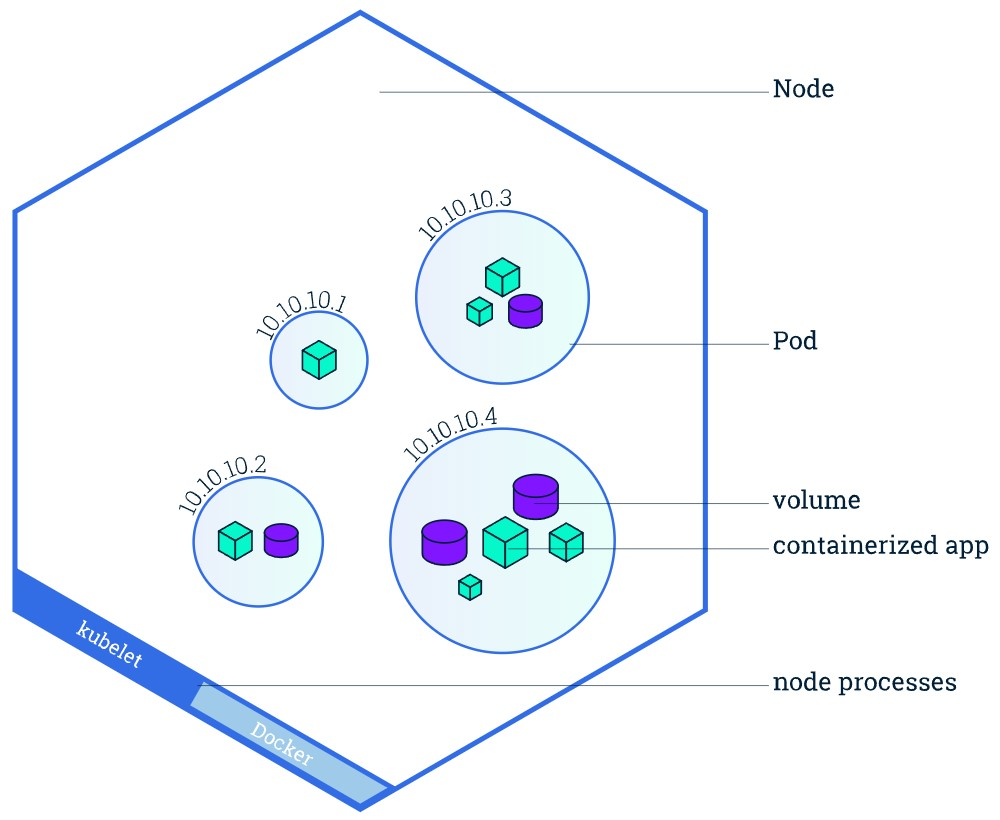
\includegraphics[width=0.6\textwidth]{img/rozdzial1-4.jpg}
    \caption{Przykładowy węzeł z czterema podami - każdy pod posiada własny adres IP dostępny wewnątrz klastra \cite{kubernetes}}
\end{figure}

Klaster (ang. \textit{cluster}) to zbiór maszyn (nazywanych węzłami, ang. \textit{nodes}), na których uruchamiane są skonteneryzowane aplikacje. Węzeł może być maszyną fizyczną lub wirtualną. Każdy klaster musi składać się z przynajmniej jednego węzła, lecz w środowisku produkcyjnym zwykle jest złożony z większej ich liczby. 

Rysunek 3.2 przedstawia przykładowy klaster działający w chmurze - jest zbudowany z trzech węzłów roboczych (ang. \textit{worker nodes}), które zarządzane są przez jeden węzeł warstwy sterowania (ang. \textit{master node}). W takiej konfiguracji węzły robocze odpowiedzialne są za uruchamianie i podtrzymywanie wdrożonych na nich aplikacji, natomiast master monitoruje stan klastra, odpowiada na jego zmieniające się parametry i komunikuje z API dostarczyciela chmury obliczeniowej. 

\begin{figure}[H]
    \centering
    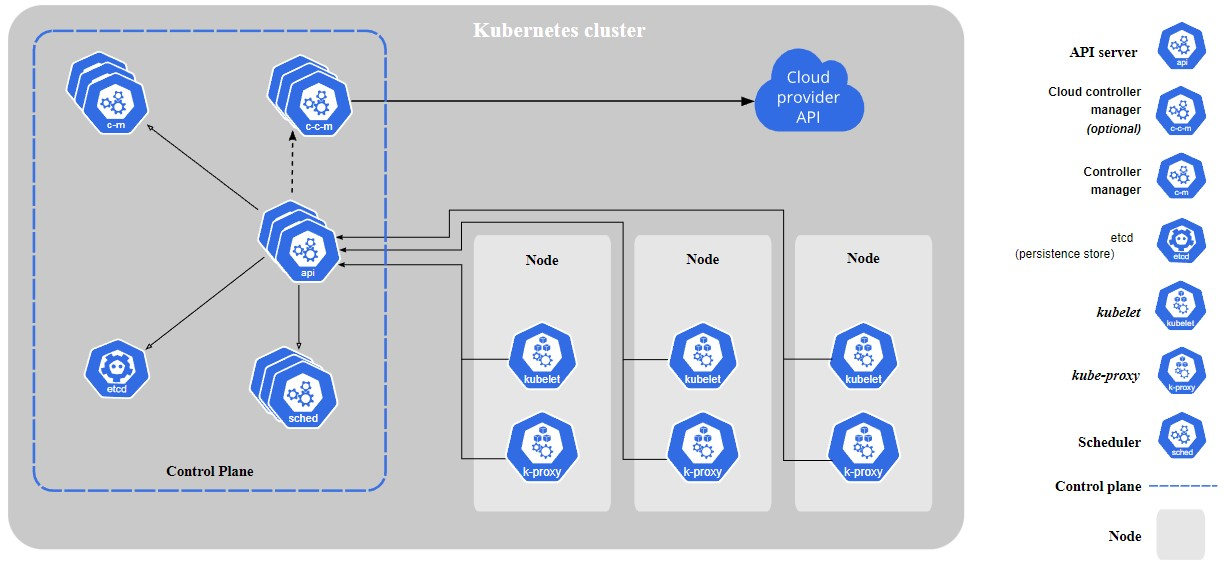
\includegraphics[width=1\textwidth]{img/rozdzial1-3.jpg}
    \caption{Części składowe przykładowego klastra Kubernetes \cite{kubernetes}}
\end{figure}

Składniki Kubernetesa uruchamiane są na każdym węźle, utrzymują działanie podów i definiują środowisko. Składowymi każdego węzła są:
\begin{itemize}
    \item kubelet - odpowiada za uruchamianie kontenerów wewnątrz poda,
    \item kube-proxy - utrzymuje reguły sieciowe węzłów, umożliwiając komunikację między podami a sieciami wewnętrznymi klastra, jak i sieciami zewnętrznymi,
    \item container runtime - oprogramowanie służące do uruchamiania kontenerów, zapewnia obsługę m.in. silnika Dockera.
\end{itemize}

Warstwa sterowania (ang. \textit{control plane}) zarządza klastrem i należącymi do niej podami. Warstwa sterowania może obsługiwać wiele rozproszonych maszyn, zapewniając niezawodność infrastruktury. 

Komponenty warstwy sterowania w wielowęzłowym klastrze zwykle uruchamiane są na osobnej maszynie, gdzie kontenery nie są uruchamiane.\\

Części składowe warstwy sterowania odpowiadają za podejmowanie decyzji oraz wykrywanie zdarzeń w klastrze. Wymienić można poniższe komponenty:

\begin{itemize}
    \item kube-apiserver - główny składnik, udostępnia API, dzięki któremu możliwa jest modyfikacja obiektów i komunikacja między nimi,
    \item etcd - przechowuje dane o klastrze, jego konfigurację i statusy usług,
    \item kube-scheduler - monitoruje tworzenie podów i przypisuje im odpowiednie węzły,
    \item kube-controller-manager - odpowiada za działanie kontrolerów - procesów, które nadzorują stan klastra i w razie potrzeby przywracają klaster do stanu oczekiwanego,
    \item cloud-controller-manager - umożliwia opcjonalne połączenie klastra z usługą chmurową.
\end{itemize}


\section{Funkcjonalności}

Spośród najważniejszych funkcjonalności Kubernetesa można wymienić:
\begin{itemize}
    \item utrzymywanie określonej liczby kontenerów na hoście zgodnej ze stanem oczekiwanym,
    \item możliwość zautomatyzowania procesu tworzenia nowych kontenerów przy wprowadzaniu zmian i zastępowania ich bez utraty dostępności,
    \item balansowanie ruchu (ang. \textit{load balancing}) w celu zapewnienia stabilności infrastruktury,
    \item wykrywanie nowych usług i udostępnianie kontenerów przy pomocy adresu IP lub DNS (ang. \textit{Domain Name System}),
    \item samonaprawa - restartowanie kontenerów, które przestały działać, badanie ich stanu i wymiana na nowe.
\end{itemize}

Kubernetes udostępnia również zestawy narzędzi służących do debugowania, monitorowania oraz zbierania logów. Jednym z nich jest Dashboard - webowy interfejs ogólnego zastosowania, w którym można uzyskać m.in. informacje o stanie klastra i wykorzystywanych zasobach \cite{kubernetes}. Poprzez interfejs możliwe jest również dodawanie nowych obiektów w klastrze oraz edycja już istniejących.
\newpage 

Rysunek 3.3 przedstawia zakładkę podów w interfejsie Dashboardu. Wyświetlona jest lista działających w klastrze podów z informacją o czasie ich działania, statusie oraz indywidualnym zużyciu pamięci oraz procesora. Powyżej listy znajdują się takżę dwa wykresy obrazujące skumulowane wykorzystanie zasobów przez pody. 
\vspace{2em}

\begin{figure}[h]
    \centering
    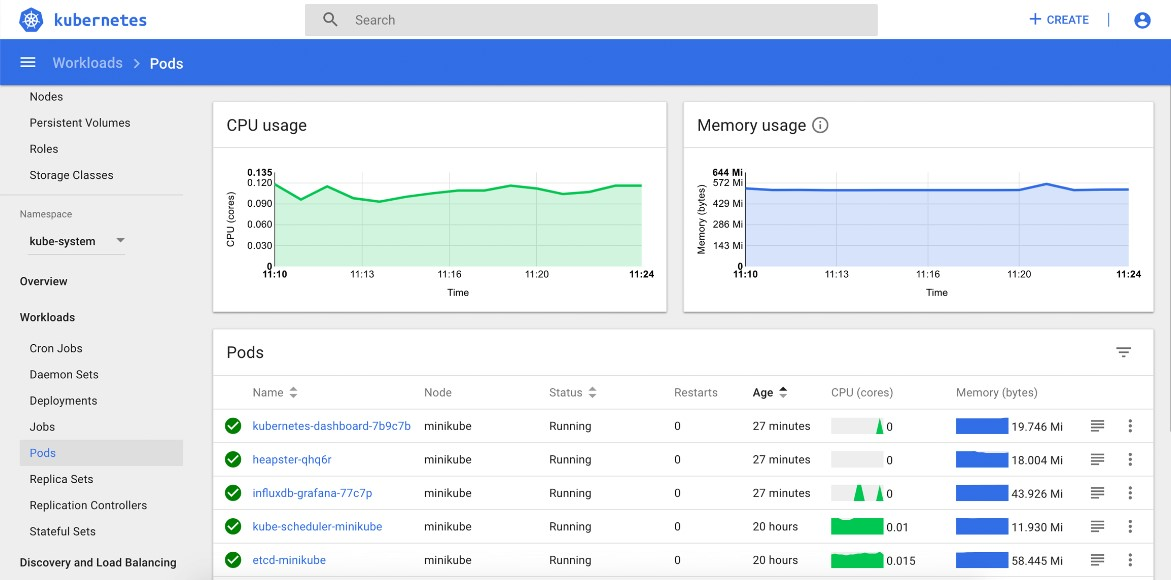
\includegraphics[width=1\textwidth]{img/rozdzial1-52.jpg}
    \caption{Kubernetes Dashboard - interfejs \cite{kubernetes}}
\end{figure}

%%%%%%%%%%%%%%%%%%%%%%%%%%%%%%%%%%%%%%%%%%


\chapter{Dodatkowe narzędzia}

Przy tworzeniu projektu wykorzystano również narzędzia open source, umożliwiające testowanie i monitorowanie klastra czy też zautomatyzowanie czynności w infrastrukturze.

\section{Automatyzacja zadań}

\begin{itemize}
    \item Helm \cite{helm} to opracowany dla Kubernetesa menedżer pakietów, który znacznie ułatwia instalację i zarządzanie wstępnie skonfigurowanymi aplikacjami. Pakiety, nazywane \textit{chart}, są tworzone i umieszczane w repozytoriach, by następnie ściągnąć je i uruchomić w środowisku klastra. Gotowe charty publikowane są na stronie internetowej Artifact Hub \cite{artifacthub}.

    %\item Ansible \cite{ansible} jest wieloplatformowym narzędziem służącym do automatyzacji zadań związanych z instalacją i konfiguracją systemów operacyjnych. W plikach YAML, zwanych \textit{playbookami}, opisywany jest stan oczekiwany systemu. Ansible umożliwia uruchamianie playbooków na wielu hostach.
\end{itemize}

\section{Monitoring}

Jako dopełnienie funkcjonalności interfejsu Kubernetes Dashboard wykorzystano poniższe platformy:

\begin{itemize}
    \item Prometheus \cite{prometheus} to zbiór aplikacji służących do zbierania i przechowywania danych szeregu czasowego oraz przesyłania alertów. Wykorzystanie bazy danych szeregów czasowych (ang. \textit{time series database}) pozwala na analizę danych w porządku czasowym i przedstawienie ich w formie wykresu, gdzie na osi X znajdują się przedziały czasu. Ponadto Prometheus oferuje własny język zapytań PromQL.

    \item Grafana \cite{grafana} służy do monitoringu i wizualizacji danych z wybranego źródła - narzędzie obsługuje większość popularnych baz danych różnego rodzaju. Grafana przedstawia zebrane dane w formie wykresów. Możliwe jest importowanie predefiniowanych dashboardów lub tworzenie własnych, co pozwala na dużą personalizację. 
\end{itemize}

\section{Testowanie}

Testy wydajnościowe mają na celu sprawdzenie badanej infrastruktury pod kątem spełnienia określonych wymagań, np. szybkości działania, dostępności itp. 

W projekcie wykorzystano dwa rodzaje testów: obciążeniowe (ang. \textit{load testing}) oraz przeciążające (ang. \textit{stress testing}). Pierwszy z nich sprawdza działanie infrastruktury przy przewidywanym obciążeniu ze strony np. użytkowników i wynikającego z tego ruchu sieciowego. Z kolei drugi wymieniony rodzaj testu polega na doprowadzeniu infrastruktury do skrajnej sytuacji, takiej jak pełne obciążenie CPU (ang. \textit{central processing unit}), pamięci itd.

Do przeprowadzenia testów wykorzystano oprogramowanie:
\begin{itemize}
    \item Narzędzie K6 \cite{k6} służy do tworzenia testów wydajnościowych, m.in. obciążenia serwisów. Skrypty testów tworzone są w języku JavaScript. Oprogramowanie pozwala na tworzenie tzw. wirtualnych użytkowników, symulujących prawdziwy ruch sieciowy. Ponadto przy pisaniu skryptów deklarowany jest czas trwania testu oraz jego fazy, w których ruch może ulec zmianie itp., co pozwala na dostosowanie testów do wymagań i charakteru infrastruktury. 

%    \item KBoom \cite{kboom} to prosty program sprawdzający szybkość i skalowalność klastra, tworząc wybraną ilość podów w interwałach. 
    
    \item Kube-Stresscheck \cite{stress} bazuje na popularnym w systemach linuxowych programie \textit{stress}, który w pętli oblicza pierwiastek kwadratowy losowych liczb. Narzędzie pozwoli sprawdzić jak zachowuje się infrastruktura i klaster pod dużym obciążeniem procesora i pamięci. 
\end{itemize}

\chapter{Pliki YAML}

W Kubernetesie istnieją dwie metody tworzenia zasobów - imperatywna oraz deklaratywna. Sposób imperatywny opiera się na używaniu pojedynczych komend i jest skuteczny w przypadku modyfikowania istniejących już obiektów, jednak mało wydajny w tworzeniu nowych. Metoda deklaratywna zakłada tworzenie plików tekstowych, zwanych również manifestami. Pliki te są zapisywane w formacie YAML i są opisem oczekiwanego stanu klastra, według którego tworzone są przez Kubernetesa kolejne obiekty. \\

W celu zautomatyzowania procesu wdrażania i udostępniania przykładowej aplikacji Nginx, stworzono dwa pliki YAML - kolejno dla deploymentu oraz dla service'u. 

Przy tworzeniu plików YAML dla obiektów Kubernetesa wymagane są cztery pola - \textit{apiVersion}, \textit{kind}, \textit{metadata} oraz \textit{spec}. W \textit{apiVersion} wprowadzana jest odpowiednia wersja API Kubernetesa, która wykorzystywana jest do stworzenia danego obiektu. Pole \textit{kind} informuje o typie tworzonego obiektu, np. deployment. W \textit{metadata} wprowadzane są dane, które pozwalają na identyfikację obiektu poprzez nazwy lub numeryczne identyfikatory. Tutaj definiowane mogą być również przestrzenie nazw. W ostatnim polu \textit{spec} wprowadzone informacje są opisem oczekiwanego stanu obiektu - używanych portów, liczby replik itd. 
\newpage

\scriptyaml{files/yamls/deployment.yaml}
\captionof{listing}{Plik YAML - \textit{deployment.yaml}}
\vspace{1em}

Pierwszy plik \textit{deployment.yaml} (Załącznik 5.1) jest opisem wdrażanej aplikacji Nginx. Deklarowana jest liczba podów, która zawsze powinna być dostępna w klastrze, a jako metodę aktualizowania deploymentu wybrano Rolling Update, co pozwala na wprowadzanie zmian bez przerw w dostępności. Podano obraz kontenera Dockera dla aplikacji Nginx i domyślnie wykorzystywany port, jak również dostępne dla poda maksima zasobów.
\newpage

\scriptyaml{files/yamls/service.yaml}
\captionof{listing}{Plik YAML - \textit{service.yaml}}
\vspace{1em}

Drugi plik \textit{service.yaml} (Załącznik 5.2) opisuje stan oczekiwany serwisu. Jako typ wybrano NodePort, co pozwala udostępniać aplikację z IP klastra i statycznym portem. Jeżeli nie wybrano portu, Kubernetes wybierze losowy port z zakresu 30000 - 32767. Deklarując port 30001 (linia 10) serwis będzie zawsze dostępny pod tym samym adresem.\\

W dalszej części pracy wykorzystywana będzie zarówno metoda deklaratywna, jak i imperatywna. Pierwsza z nich będzie służyć do szybkiego, automatycznego uruchamiania serwisów w klastrze, z kolei sposób imperatywny stosowany będzie do modyfikowania działających już deploymentów.


%%%%%%%%%%%%%%%%%%%%%%%%%%%%%%%%%%%%%%%%%%


\chapter{Klaster z jednym węzłem}

Przed przystąpieniem do realizacji pracy wymagana była instalacja następujących bibliotek i narzędzi na komputerze-gospodarzu:

\begin{itemize}
    \item Vagrant,
    \item \textit{qemu-kvm},
    \item \textit{libvirt},
    %\item Ansible.
\end{itemize}

Ponadto niezbędne było otwarcie portów, które w poźniejszym etapie wykorzystywane były do przekierowania udostępnionych aplikacji jako serwisu (Rysunek 6.1):

\begin{itemize}
    \item 8001 dla Kubernetes Dashboard,
    \item 30001 dla Nginx,
    \item 30002 dla Prometheusa,
    \item 30003 dla Grafany.
\end{itemize}

\begin{figure}[htp]
\makebox[\textwidth][c]{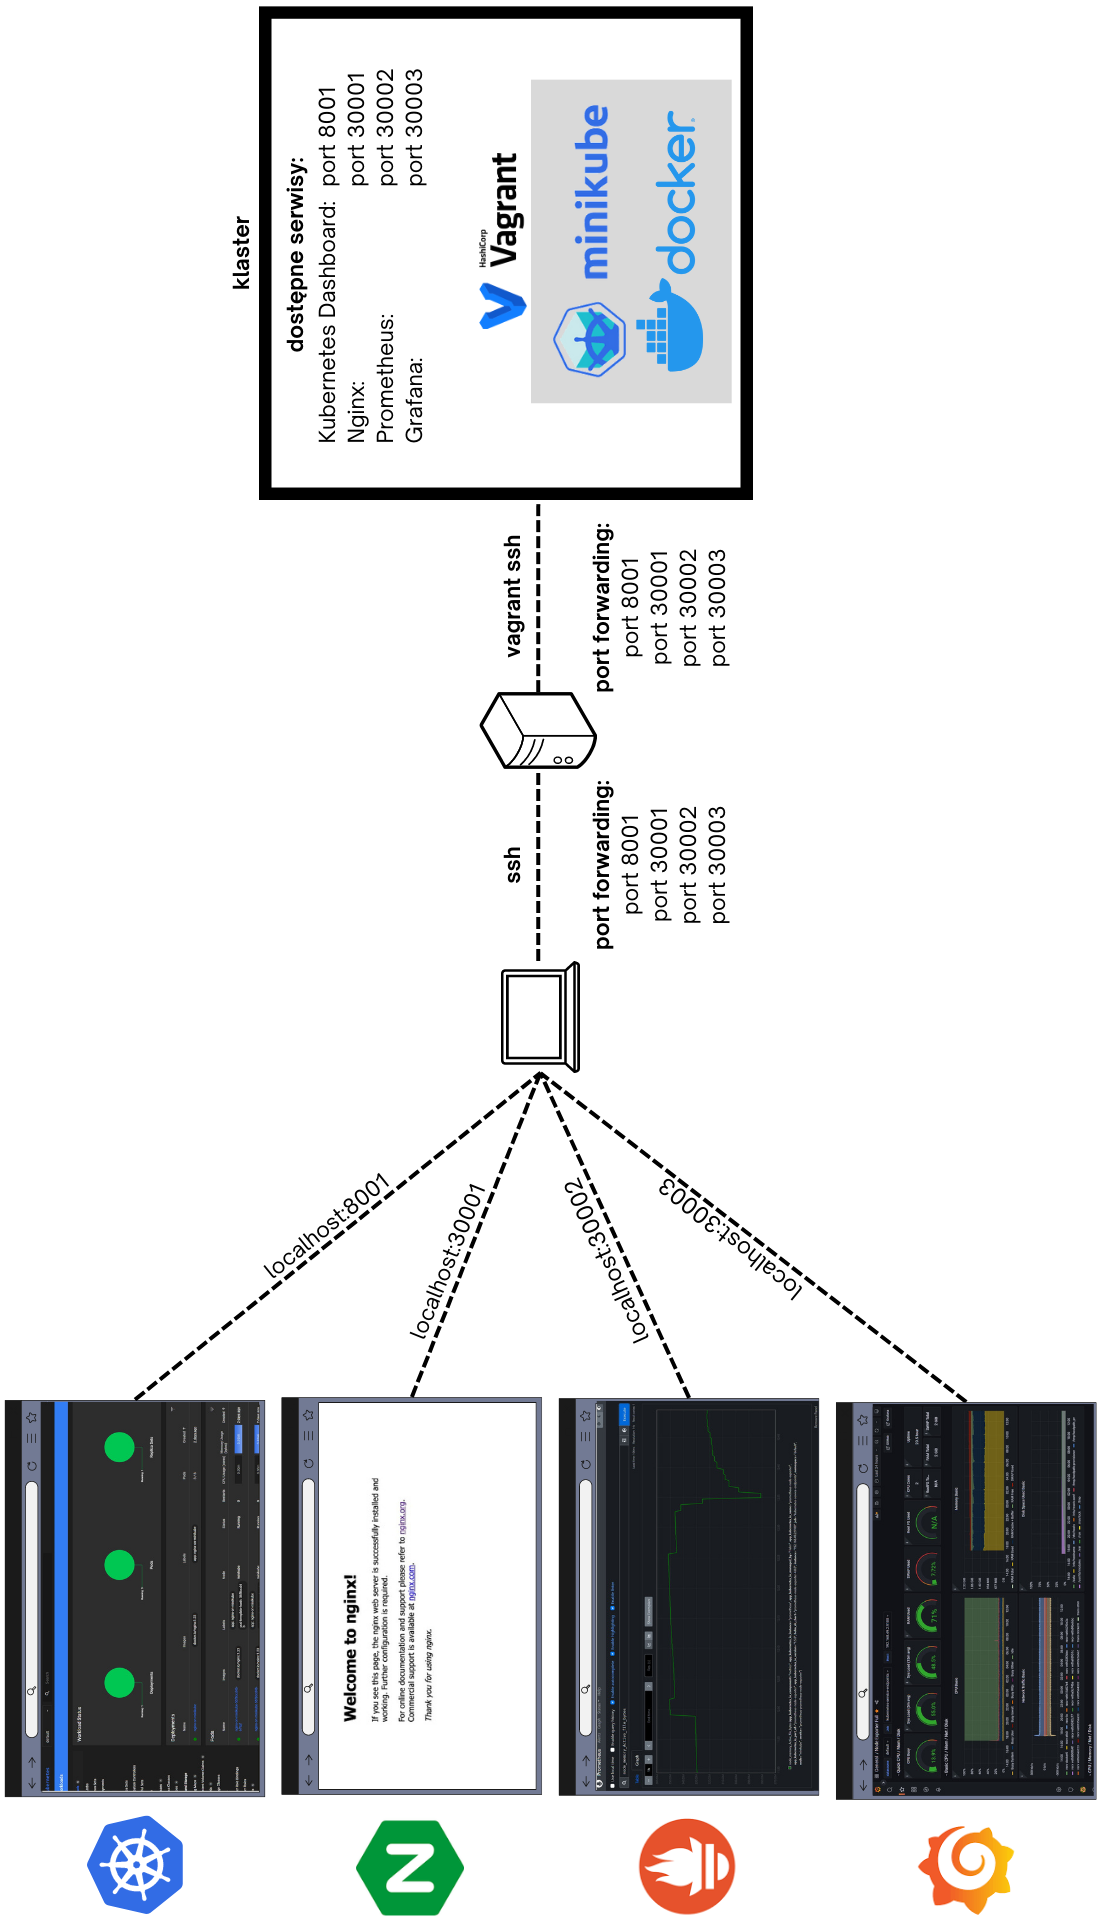
\includegraphics[width=0.95\textwidth]{img/1node.png}}
\caption{Schemat poglądowy infrastruktury dla jednego węzła}
\end{figure}
\newpage

Do stworzenia klastra z tylko jednym węzłem wybrano Minikube, który został stworzony z myślą o lokalnych, jednowęzłowych klastrach \cite{minikube}. Jako domyślne środowisko uruchamiania kontenerów w tworzonym klastrze wykorzystano natomiast Dockera. 

W celu odseparowania procesów klastra od maszyny fizycznej zdecydowano o rozwijaniu projektu wewnątrz maszyny wirtualnej. Mając na uwadze wysoką automatyzację procesu tworzenia i niszczenia kolejnych instancji maszyn, wybrano Vagranta z rozszerzeniem \textit{libvirt}, które umożliwia natywną dla Linuxa wirtualizację poprzez KVM/QEMU.\\

Pierwszym etapem pracy było utworzenie plików konfiguracyjnych służących do zautomatyzowania procesu uruchomienia maszyny wirtualnej i tworzenia samego klastra. W pliku \textit{Vagrantfile} (załącznik 9.1) zdefiniowano najważniejsze właściwości maszyny - przekierowania portów oraz dostępne zasoby, takie jak pamięć oraz rdzenie procesora. Jako system operacyjny wybrano Ubuntu 20.04 LTS. Ponadto wykorzystano funkcjonalność \textit{provision}, która pozwala zainstalować predefiniowane przez Vagranta narzędzia w szybki i prosty sposób - w tym przypadku Dockera.

W kolejnym kroku utworzono skrypt powłoki systemowej Bash - \textit{config.sh} (Załącznik 9.2), który umożliwia instalację narzędzi służących do kontrolowania i zarządzania klastrem - Minikube oraz Kubectl. Skrypt automatyzuje również proces instalacji menedżera pakietów Helm oraz narzędzia testowego K6. 

Następnie ściągane jest repozytorium z GitHuba, składające się z plików YAML i skryptu.
Skrypt \textit{after\_config.sh} (Załącznik 9.3) uruchamia klaster poprzez wywołanie funkcji \textit{run\_minikube}. Włączany jest również Metrics Server, który zbiera dane o wykorzystaniu pamięci i CPU w klastrze oraz jest niezbędny przy autoskalowania aplikacji.

Pliki YAML dla deplyomentu (Załącznik 5.1) oraz service'u (Załącznik 5.2) pozwalają na szybkie wdrożenie aplikacji Nginx, która jest uruchamiana w klastrze. Następnie instalowane i uruchamiane są narzędzia służące do zbierania danych i monitoringu klastra - Prometheus i Grafana.\\

Używając komendy \textit{vagrant up} rozpoczynany jest proces tworzenia i konfigurowania maszyny wirtualnej. Po zakończeniu działania skryptów, maszyna jest gotowa do działania i możliwe jest połączenie się z nią, używając \textit{vagrant ssh} w tym samym katalogu, w którym została stworzona.

W dalszej konfiguracji jednowęzłowego klastra konieczna jest manualna interwerncja administratora. Interfejs Kubernetes Dashboard uruchamiany jest poprzez \textit{minikube dashboard}. Należy również umożliwić zdalny dostęp poprzez polecenie \textit{kubectl proxy}, co pozwoli na podgląd interfejsu w przeglądarce z komputera spoza sieci klastra. Podobnie w przypadku utworzonych serwisów Nginx, Prometheusa i Grafany - aby móc do nich przejść spoza tej samej sieci, konieczne jest otwarcie portów, używając komendy \textit{kubectl port-forward} i podając adekwatny port. 

Ostatnim etapem jest skonfigurowanie Grafany - aby uzyskać dostęp do platformy, należy pozyskać hasło (Załącznik 9.3, linia 47). Następnie po zalogowaniu dodajemy źródło danych, w tym przypadku Prometheusa. Aby wyświetlić zebrane przez niego informacje, importujemy dashboard (np. Node Exporter Full \cite{nodeexporterfull}).\\

W ten sposób utworzona maszyna wirtualna jest przygotowana do dalszych działań i testów.

%%%%%%%%%%%%%%%%%%%%%%%%%%%%%%%%%%%%%%%%%%

\section{Podstawowe operacje w klastrze}

Po skonfigurowaniu klastra możliwe jest sprawdzenie działających w nim zasobów, co można uczynić wewnątrz maszyny wirtualnej lub poprzez Kubernetes Dashboard.

Za pomocą komendy \textit{kubectl get pods} wylistowane są wszystkie pody w klastrze, również te, które nie mogą zostać uruchomione - wówczas w trzeciej kolumnie pojawia się informacja ze stosownym statusem. 
W przypadku omawianej infrastruktury wszystkie pody zostały uruchomione i żaden nie był restartowany przez Kubernetesa (Rysunek 6.2). 

\begin{figure}[h]
    \centering
    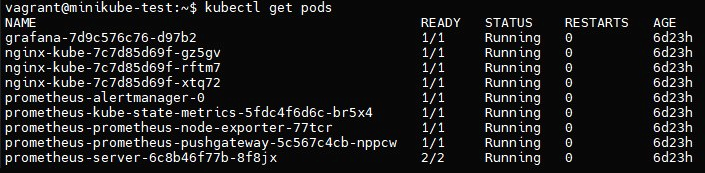
\includegraphics[width=1\textwidth]{img/basic1.png}
    \caption{Wynik komendy \textit{kubectl get pods}}
\end{figure}
\newpage

Można również zauważyć, że Kubernetes utworzył 3 pody nginx-kube - zgodnie z manifestem \textit{deployment.yaml}. 

Aby sprawdzić szczegóły utworzonego serwisu nginx-kube (Rysunek 6.3), w terminalu można użyć komendy: 
%$\textit{kubectl describe svc nginx-kube}
\scriptbash{files/minikube/commands/svc.txt}

\begin{figure}[h]
    \centering
    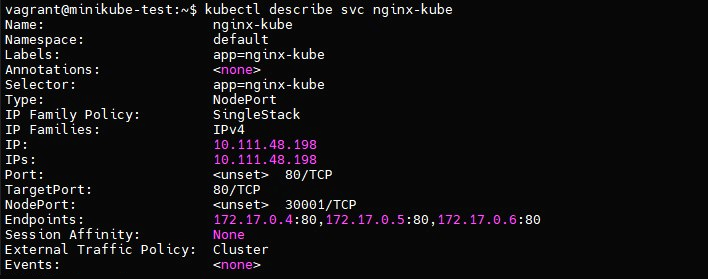
\includegraphics[width=1\textwidth]{img/basic2.png}
    \caption{Wynik komendy \textit{kubectl describe svc nginx-kube}}
\end{figure}

Kubernetes przypisał serwisowi unikalny wewnątrz klastra adres IP. Ponadto poszczególne porty zostały przypisane na podstawie deklaracji zawartych w pliku \textit{service.yaml}. Port 80 oraz TargetPort 80 są odsłonięte do komunikacji z podami wewnątrz klastra, z kolei NodePort 30001 odsłania serwis poza klastrem i umożliwia dostęp do niego. 

Endpoints to adresy IP podów. Przy tworzeniu service'u Kubernetes przypisał ww. trzy pody do powstałego service'u. Pozwala to, by ruch przychodzący do serwisu nginx-kube, przekierowany był do któregoś z podów. 

%Service aplikacji posiada również External Traffic Policy z domyślnym ustawieniem na Cluster. Dzięki tej opcji Kubernetes będzie przekazywał ruch do każdego poda działającego w ramach serwisu, niezależnie od tego na jakim węźle się znajduje, co zaobserwowane będzie w przypadku klastra z dwoma węzłami. 
 
\section{Równoważenie obciążenia}

Równoważenie obciążenia to metoda rozproszenia obciążenia między wiele zasobów. W przypadku serwisów Kubernetes będzie starał się równomiernie rozdystrybuować przychodzący ruch między działające pody. Jedną z metod jest zaimplementowany w module kube-proxy algorytm karuzelowy (ang. \textit{round robin}). 

W celu sprawdzenia działania tego mechanizmu, stworzony został prosty skrypt \textit{curl\_120s.sh} (Załącznik 9.4), w którym co dwie minuty uruchamiana jest komenda \textit{curl} z adresem serwisu nginx-kube.

Obserwując \textit{CPU usage} w Kubernetes Dashboard (Rysunek 6.4) można zauważyć chwilowy wzrost zużycia CPU przez każdy pod, generowany przez ruch sieciowy przekierowany do podów po użyciu skryptu \textit{curl\_120s.sh}.

\begin{figure}[h]
    \centering
    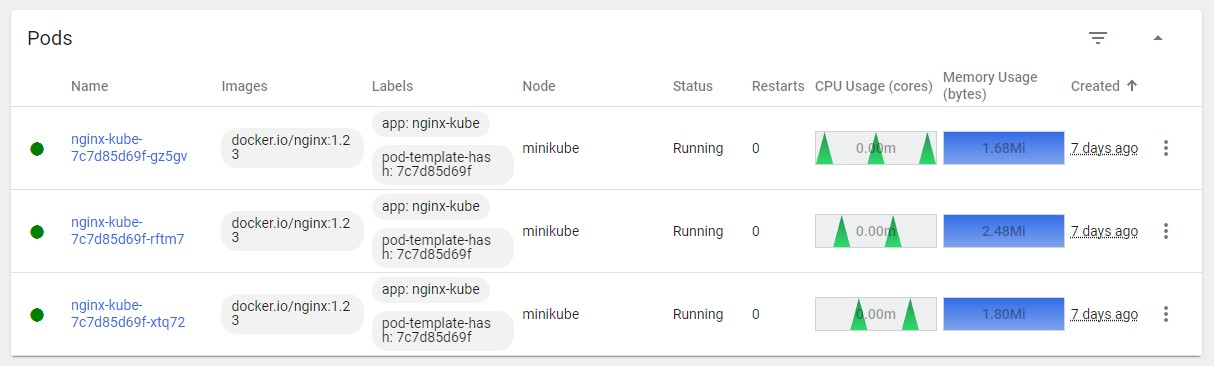
\includegraphics[width=1\textwidth]{img/load1.jpg}
    \caption{Wzrost zużycia CPU przez każdy pod po uruchumieniu \textit{curl\_120s.sh}}
\end{figure}

Logi z wybranego poda (Rysunek 6.5) potwierdzają, że ruch był kierowany cyklicznie do tego samego poda co sześć minut. 

\begin{figure}[h]
    \centering
    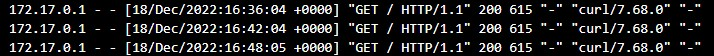
\includegraphics[width=1\textwidth]{img/load2.jpg}
    \caption{Logi poda nginx-kube-7c7d85d69f-gz5gv po użyciu skryptu \textit{curl\_120s.sh}}
\end{figure}

\section{Aktualizowanie aplikacji}

Ważną funkcjonalnością Kubernetesa jest możliwość aktualizowania deploymentu bez zakłócania pracy aplikacji, czyli tzw. \textit{rolling updates}. Wówczas wprowadzanie wszelkich zmian nie ma wpływu na dostępność serwisu. W czasie dokonywania zmian w deploymencie działanie podów jest po kolei kończone, a zastępują je nowe pody, stworzone zgodnie z zawartością aktualizacji. 

Dodatkowe parametry rolling updates zostały zdefiniowane w pliku \textit{deployment.yaml} (Załącznik 5.1). Opcja maxSurge z wartością ustawioną na 1 (linia 13) oznacza, że w trakcie aktualizacji Kubernetes może stworzyć jeden dodatkowy pod, wykraczający poza limit replik. Następna opcja - maxUnavailable o wartości 0 (linia 14) oznacza, że aktualizując deployment, minimalna liczba dostępnych podów musi być równa liczbie zadeklarowanych w manifeście replik. Wynika zatem, że stosując tego typu konfigurację, w trakcie deploymentu pracę może rozpocząć czwarty pod.

\newpage
Po uruchomieniu skryptu \textit{k6\_fast\_load.js} (Załącznik 9.5), który łącząc się z adresem serwisu, przez 2 minuty generuje rosnący ruch ze stoma użytkownikami w szczytowym momencie, dokonywana jest aktualizacja deploymentu nginx-kube poprzez polecenie:

%\textit{kubectl set image deployment.v1.apps/nginx-kube nginx=nginx:1.16.1}\\

\scriptbash{files/minikube/commands/rolling.txt}

Do deploymentu przekazywany jest obraz z inną wersją aplikacji Nginx, w tym przypadku 1.16.1. Po wprowadzeniu komendy Kubernetes od razu przechodzi do aktualizowania - kończona jest praca działających do tej pory podów i kolejno tworzone są nowe, co można obserwować w czasie rzeczywistym w Kubernetes Dashboard (Rysunek 6.6) lub używając komendy \textit{kubectl get pods} w  terminalu (Rysunek 6.7). 

\begin{figure}[h]
    \centering
    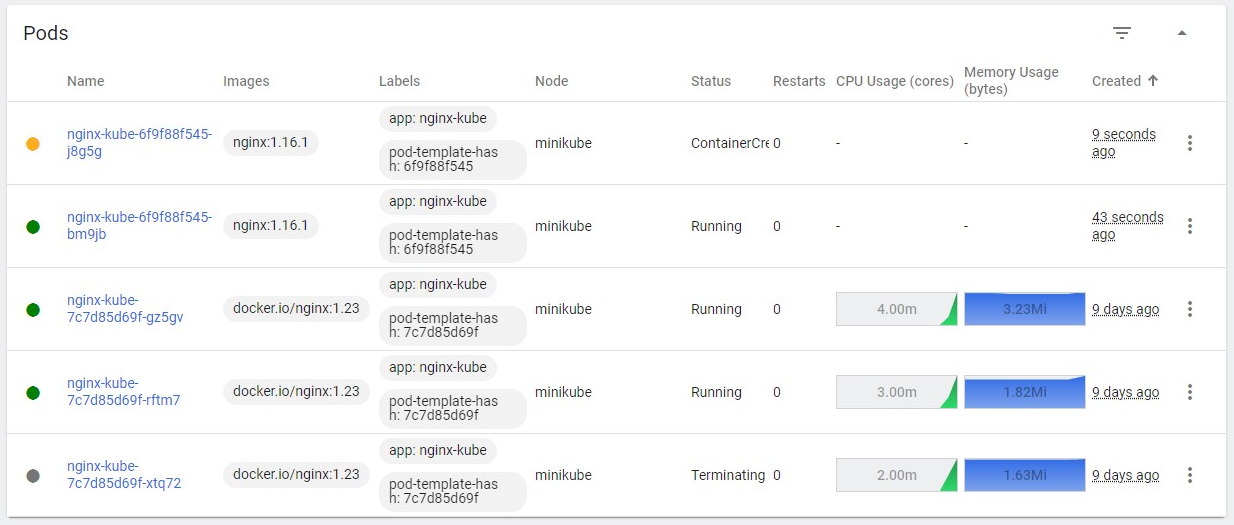
\includegraphics[width=1\textwidth]{img/roll2.png}
    \caption{Zatrzymywanie i uruchamianie podów w trakcie rolling update'u widziane w Kubernetes Dashboard}
\end{figure}

\begin{figure}[h]
    \centering
    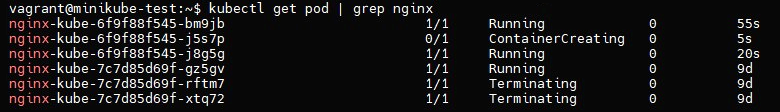
\includegraphics[width=1\textwidth]{img/roll1.png}
    \caption{Pody deploymentu nginx-kube w trakcie rolling updates - wylistowane przy pomocy komendy \textit{kubectl get pod | grep nginx}}
\end{figure}

Po zakończeniu procedury każde wejście do serwisu przekierowuje użytkownika do zaktualizowanego poda w serwisie. \\

\iffalse
        Używając platformy Prometheus oraz zapytań PromQL, wygenerowane zostały dwa wykresy - oba przedstawiające zmieniające się parametry podów z określonego zakresu czasowego, w którym dokonywana była aktualizacja. 
        
        Pierwszy z nich (Rysunek 6.8) przedstawia wszystkie działające pody (tj. te, które posiadają status \textit{Running}). Nowe pody powstawały w następstwie zmiany statusu ich poprzedników na \textit{Terminating}.  
        
        Z kolei drugi wykres (Rysunek 6.9) przedstawia zużycie procesora przez pody - zauważalne są momenty powstania nowych podów oraz ostatecznego zniszczenia podów ze starą wersją aplikacji.
        
        \begin{figure}[H]
            \centering
            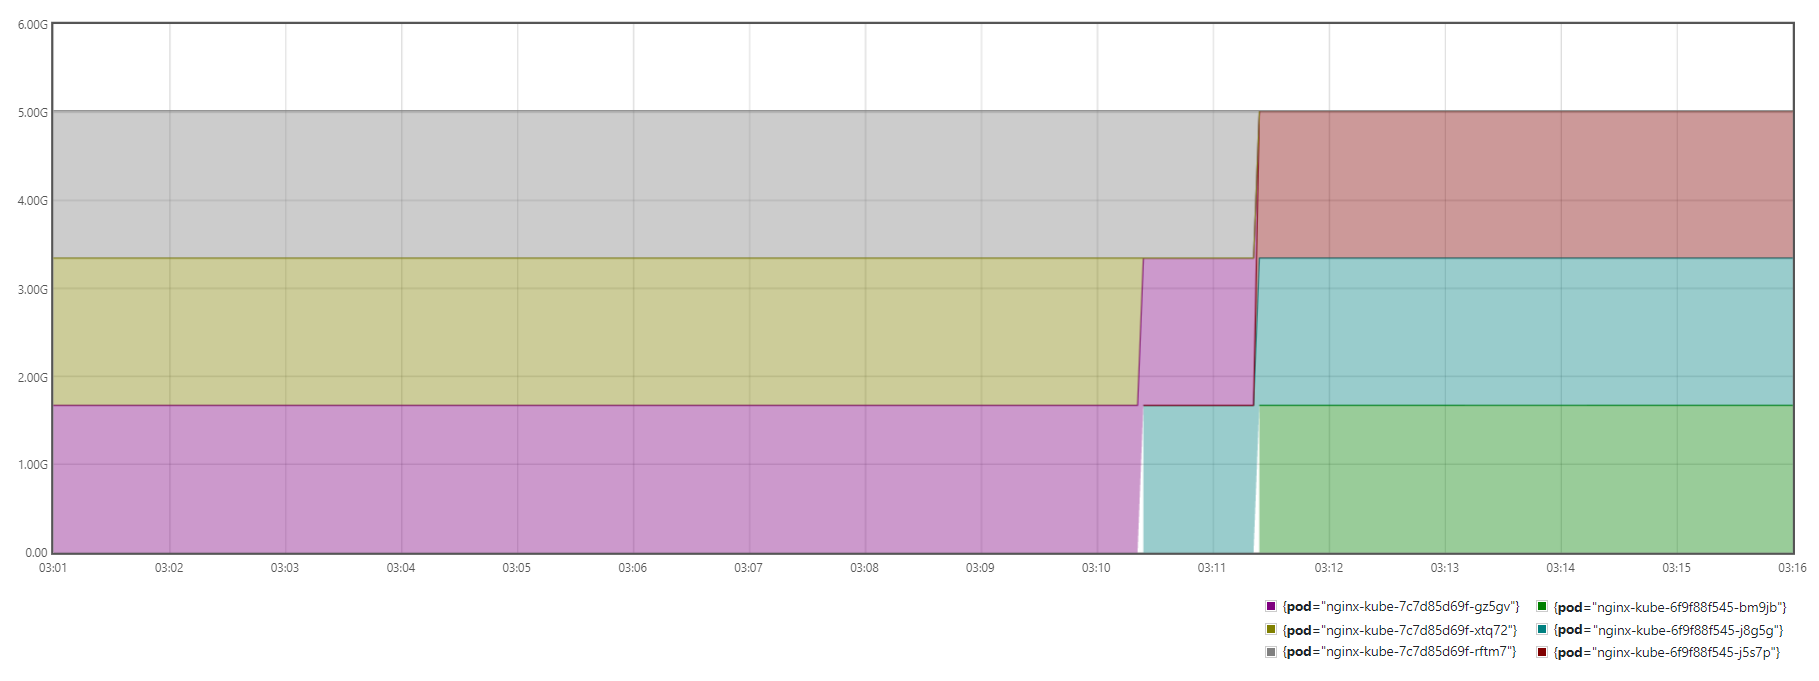
\includegraphics[width=1\textwidth]{img/roll3.png}
            \caption{Wykres skumulowany dla działających podów, zapytanie PromQL \textit{kube\_pod\_container\_status\_running\{pod=\textasciitilde\"\ nginx-kube-.*"\}}}
        \end{figure}
        
        \begin{figure}[h]
            \centering
            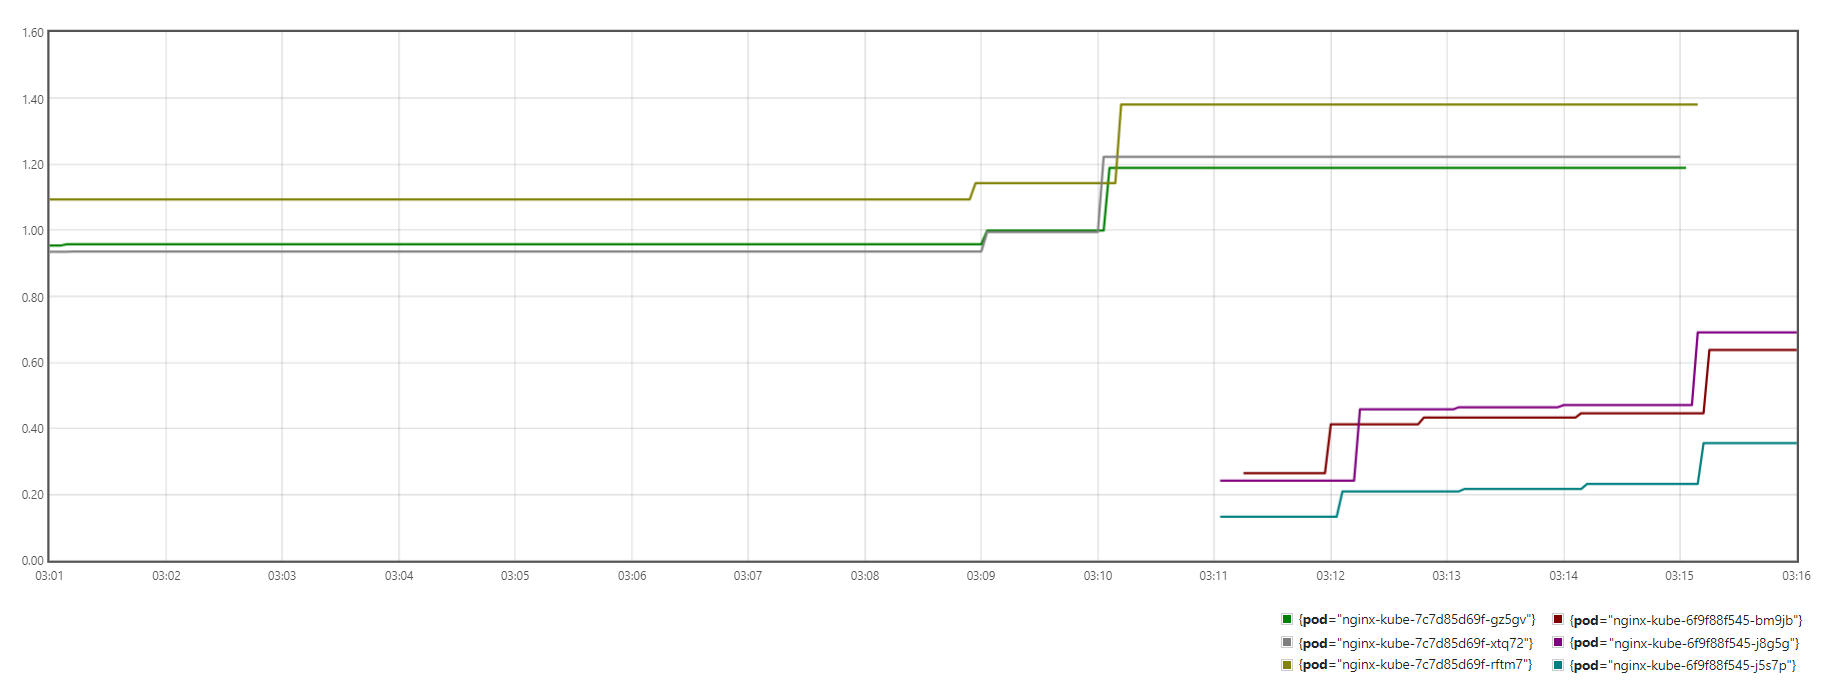
\includegraphics[width=1\textwidth]{img/roll5.png}
            \caption{Wykres przedstawia wykorzystanie procesora przez pody, zapytanie PromQL \textit{kube\_pod\_container\_status\_running\{pod=\textasciitilde\"\ nginx-kube-.*"\}}}
        \end{figure}
\fi

Używając zapytań PromQL oraz platformy Grafana, wygenerowany został wykres, przedstawiający zmieniające się zużycie CPU przez pody w czasie, gdy dokonywana była aktualizacja aplikacji (Rysunek 6.8). 

Nowe pody powstawały w następstwie zmiany statusu ich poprzedników na \textit{Terminating}. Zauważalne są momenty powstania nowych podów oraz ostatecznego zniszczenia tych ze starą wersją aplikacji - wówczas dane o użyciu procesora przestają pojawiać się na wykresie.

\begin{figure}[H]
    \centering
    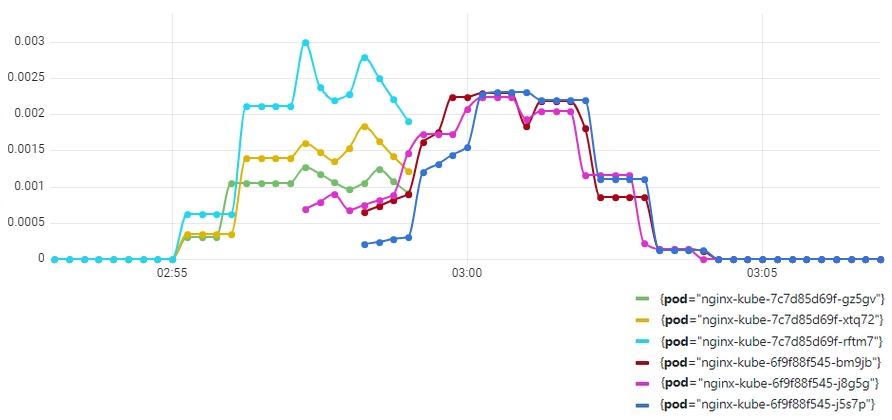
\includegraphics[width=1\textwidth]{img/cpu_rolling.jpg}
    \caption{Wykres zużycia rdzeni CPU przez pody dla zapytania PromQL \textit{rate(container\_cpu\_usage\_seconds\_total\{pod=\textasciitilde\"\ nginx-kube-.*"\}[4m])}}
\end{figure}

\section{Skalowanie horyzontalne}

Na etapie deploymentu aplikacji zadeklarowano, że liczba replik podów zawsze będzie wynosić trzy (Załącznik 5.1, linia 9). Oznacza to, że niezależnie od obciążenia serwisu, ruch obsługiwany będzie przez trzy pody. W przypadku zwiększenia obciążenia dostęp do serwisu może stać się utrudniony dla użytkowników, skąd wynika potrzeba autoskalowania.\\

Skalowanie horyzontalne w Kubernetesie znane jest jako Horizontal Pod Autoscaler lub w skrócie HPA. Dzięki tej funkcjonalności Kubernetes jest w stanie dynamicznie zmieniać liczbę działających podów, biorąc pod uwagę wykorzystane zasoby. HPA pozwala zatem minimalizować ryzyko przeciążeń systemu, dostosowując liczbę podów względem bieżących potrzeb.

Działanie Horizontal Pod Autoscalera oparte jest o pętlę, zbierającą w określonych odstępach (domyślnie co 15 sekund) informacje o zasobach. Aby to wykonać niezbędne jest uruchomienie Metrics Server, zbierającego parametry klastra (Załącznik 9.3, linia 5). Korzystając z danych, obliczana jest oczekiwana liczba replik, a następnie Kubernetes dostosowuje liczbę podów.\\

W celu wdrożenia HPA dla deploymentu nginx-kube wykorzystano metodę imperatywną, wpisując w terminalu:
%\textit{kubectl autoscale deployment nginx-kube -{}-min=3 -{}-max=10 -{}-cpu-percent=60}\\

\scriptbash{files/minikube/commands/hpa.txt}

Trzy pody pozostają minimalną liczbą działających podów, natomiast ich maksymalna liczba przy największym obciążeniu wynosi dziesięć. Autoskalowanie zaczyna tworzyć nowe pody przy obciążeniu CPU wynoszącym 60\% zadeklarowanej wartości request (Załącznik 5.1, linia 34). 
%Oznacza to, że jeśli ruch przychodzący do podów będzie na tyle duży, że każdy pod wykorzysta pulę dostępnych dla niego zasobów, to stworzony zostanie nowy pod.

Wówczas proces tworzenia kolejnych podów rozpoczynany jest natychmiast, natomiast w przypadku spadku ruchu pody są domyślnie niszczone w przeciągu 300 sekund.\\

Skrypt \textit{k6\_long\_load.js} (Załącznik 9.6) umożliwa sprawdzenie działania HPA. Po uruchomieniu K6 generuje początkowo wzrastający ruch z maksimum 300 użytkowników, który następnie stopniowo maleje.

W pierwszej fazie wzrastania liczby użytkowników utworzonych zostało 7 nowych podów (Rysunek 6.9).

\begin{figure}[H]
    \centering
    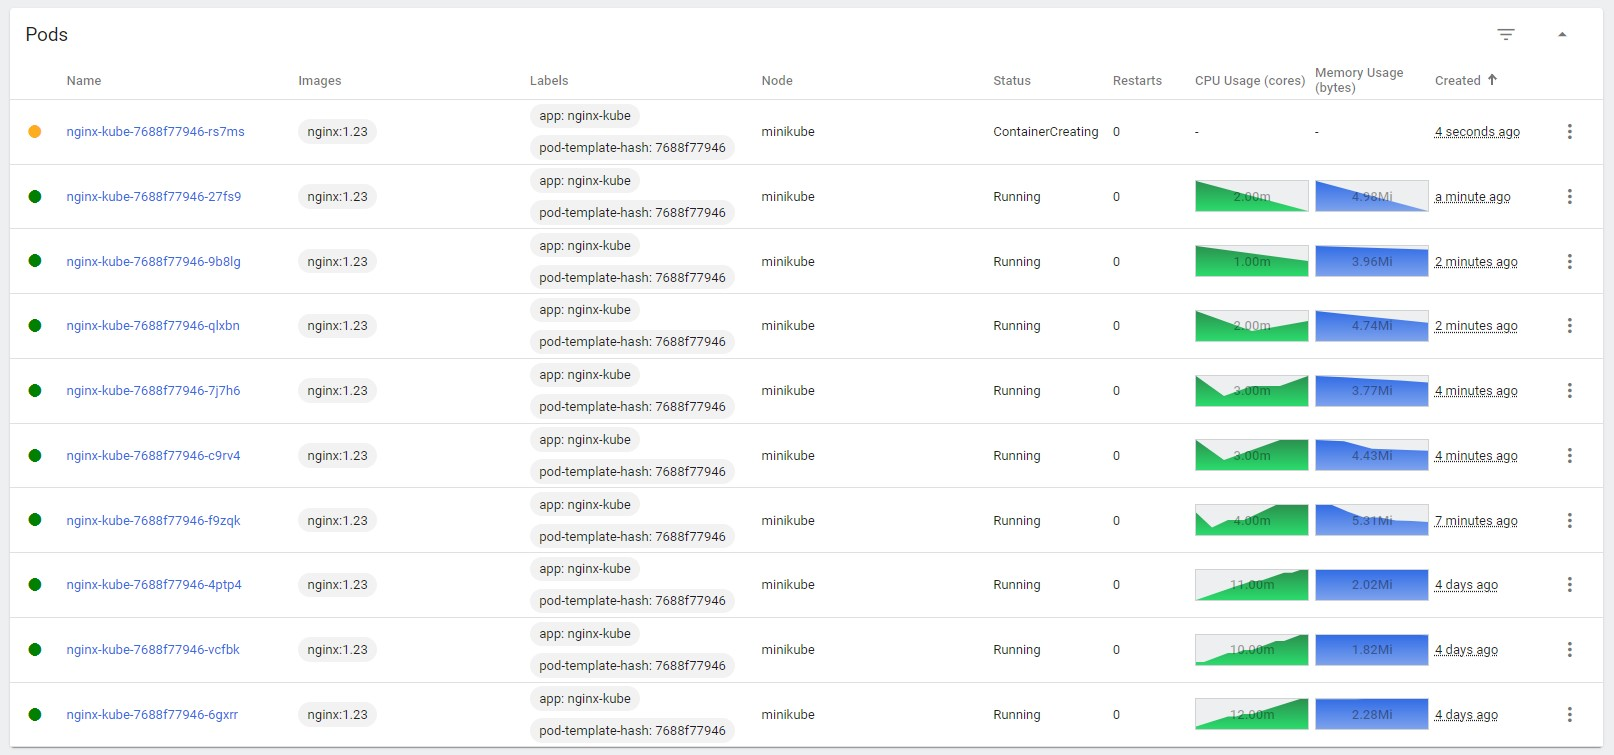
\includegraphics[width=1\textwidth]{img/hpa.jpg}
    \caption{Pody utworzone przez HPA w Kubernetes Dashboard}
\end{figure}
\newpage

Natężenie ruchu utrzymywało stałą liczbę podów, by następnie wraz ze spadkiem liczby wirtualnych użytkowników dostających się do serwisu, najnowsze pody były przez Kubernetesa wyłączane. Wykres (Rysunek 6.10) przedstawia zmiany w zużyciu procesora przez pody w trakcie pięćdziesięciu minut działania skryptu \textit{k6\_long\_load.js} i obrazuje działanie Horizontal Pod Autoscalera. 

\begin{figure}[H]
    \centering
    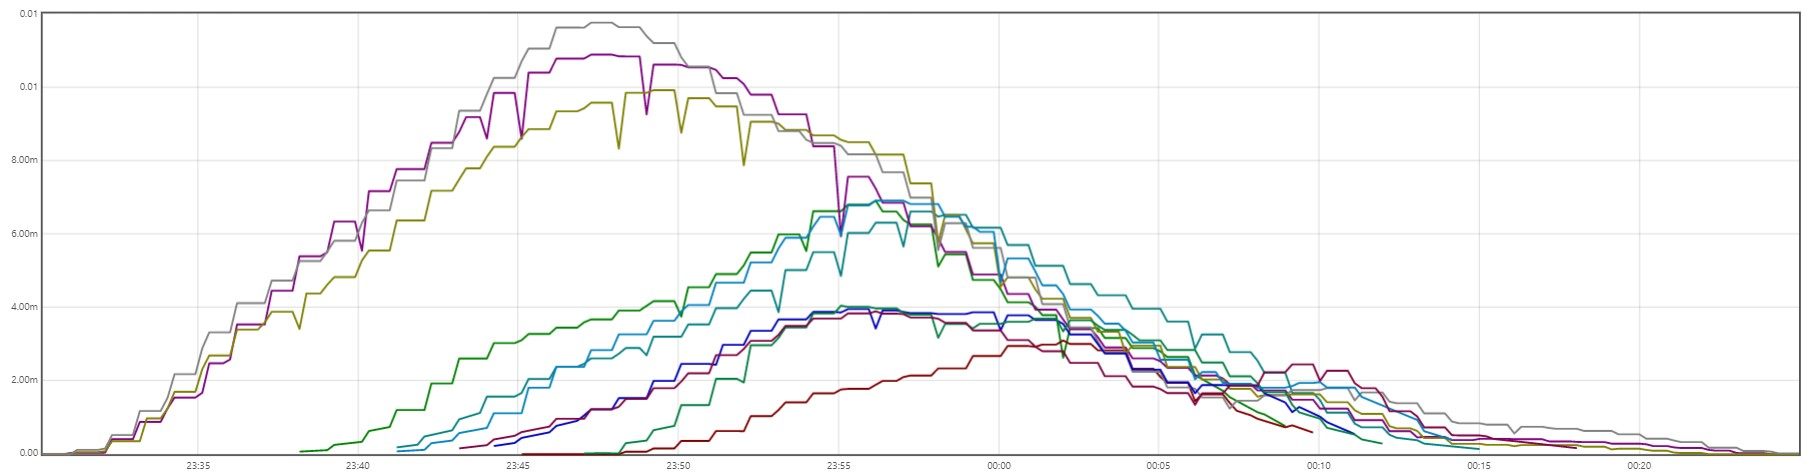
\includegraphics[width=1\textwidth]{img/hpa_d.jpg}
    \caption{Zużycie CPU a tworzenie nowych podów - zapytanie PromQL \textit{rate(container\_cpu\_usage\_seconds\_total\{pod=\textasciitilde \"\ nginx-kube-.*"\}[5m])}}
\end{figure}


\section {Testowanie wydajności klastra z jednym węzłem}

Na wydajność infrastruktury i klastra składa się wiele czynników, spośród którym można wyróżnić:

\begin{itemize}
    \item rodzaj maszyny - fizyczna lub wirtualna,
    \item \textit{workload} serwera - liczba zadań wykonywanych przez ten sam komputer,
    \item ilość dostępnych dla maszyny zasobów,
    \item wydajność samych podzespołów,
    \item przepustowość łącza,
    \item działanie obsługiwanych aplikacji.
\end{itemize}

Przy projektowaniu infrastruktury należy brać pod uwagę przewidywany ruch sieciowy ze strony użytkowników i możliwe tym samym skoki w natężeniu wejść na udostępnianą usługę. Tego typu skoki mogą powodować poważne problemy w nieprzygotowanym do tego komputerze, prowadząc nie tylko do przerwania działania aplikacji, ale również do zawieszenia pracy całego systemu. 

Dzięki przeprowadzaniu testów wydajnościowych sprawdzane są możliwości maszyny i jej działanie, co pozwala na wprowadzenie ewentualnych modyfikacji przed udostępnieniem jej dla użytkowników. 

W przypadku tworzonego w pracy klastra oraz maszyny wirtualnej głównym celem testów było wyszukanie tzw. "wąskich gardeł", czyli elementów infrastrukty wykazujących niższą od pozostałych sprawność, które powodują znaczny spadek wydajności.\\

Pierwszy test \textit{k6\_test\_cluster.js} (Załącznik 9.7) polegał na symulowaniu napływającego ruchu sieciowego użytkowników do serwisu nginx-kube, używając do tego oprogramowania K6.
Przez pierwsze dwadzieścia minut tworzonych jest 600 wirtualnych użytkowników, co daje stały przypływ 30 użytkowników na minutę. Przez następne 10 minut utrzymywany jest ruch 600 userów. W przeciągu kolejnych 15 minut ruch wzrasta do 800 użytkowników, po czym spada do zera. 

Następnym etapem testu jest sprawdzenie jak duża i gwałtowna zmiana we wzroście ruchu sieciowego wpływa na maszynę - w trakcie trzech minut liczba wirtualnych użytkowników rośnie od zera do tysiąca. Ostatecznie ruch spada do stu userów i utrzymuje się kilka minut, aż jakikolwiek ruch do serwisu ustaje.\\

Po zakończeniu działania skryptu \textit{k6\_test\_cluster.js} wykorzystano Grafanę w celu przeanalizowania wyników testu. Wykorzystano zarówno predefiniowane wykresy dashboardu Node Exporter Full, jak również stworzono nowe. Wszystkie poniższe wykresy przedstawiają przedział czasowy od godziny 13:50 do 15:10. Dodatkowo niebieską, przerywaną linią oznaczono przybliżony czas działania ww. skryptu, tj. uruchomienie narzędzia K6 o godzinie 14:00 oraz koniec działania skryptu o 15:00.\\

Rysunek 6.11 przedstawia ruch sieciowy - przychodzący i wychodzący. Największe amplitudy widoczne są w przypadku połączeń z głównym interfejsem sieciowym \textit{eth0}, który używany jest przez wirtualną maszynę, oraz \textit{docker0}, mostu używanego przez Dockera. Most ten łączy sieć maszyny z siecią klastra poprzez wirtualne interfejsy \textit{veth}, które obsługują działające w klastrze kontenery.

\begin{figure}[H]
    \centering
    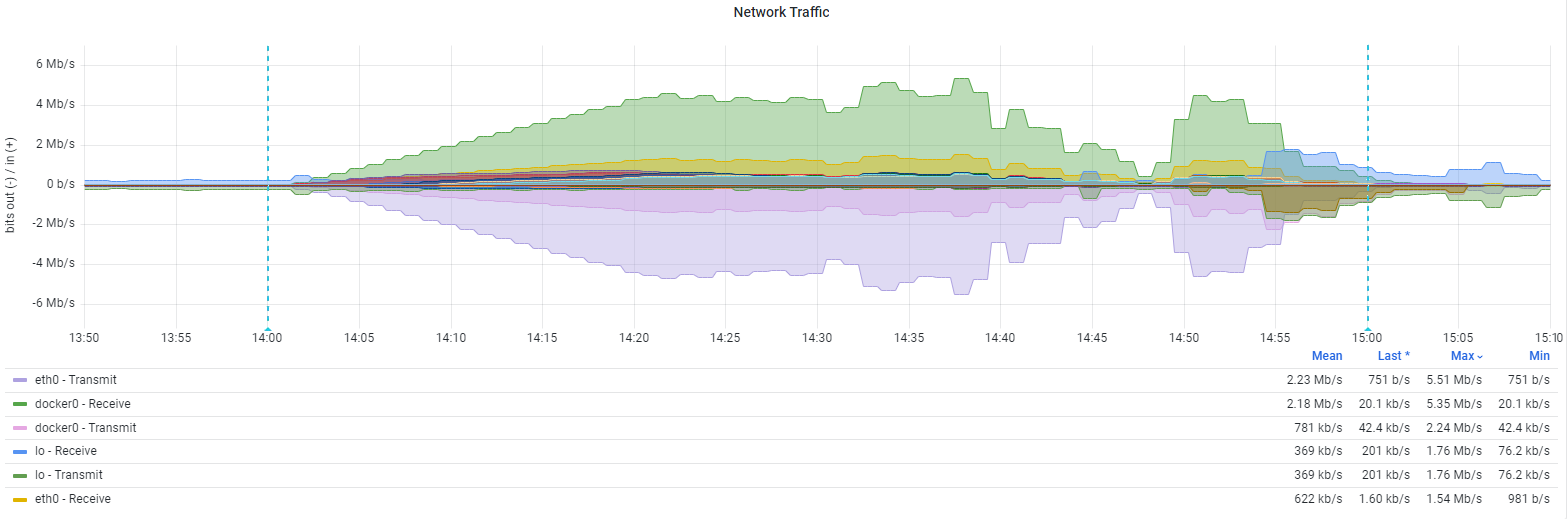
\includegraphics[width=1\textwidth]{img/test_one/network111.png}
    \caption{Wykres przedstawiający ruch przychodzący i wychodzący w sieci wirtualnej maszyny}
\end{figure}


%    \begin{figure}[H]
%       \centering
%       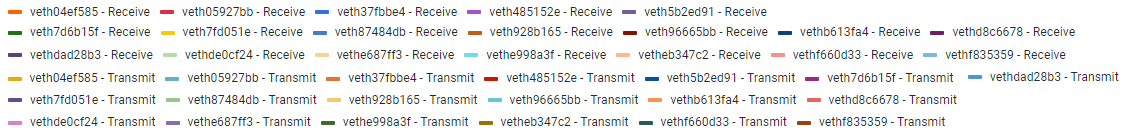
\includegraphics[width=1\textwidth]{img/test_one/recvtrans.png}
%       \caption{Wirtualne interfejsy sieciowe obsługujące klaster w trakcie działania skryptu \textit{k6\_test\_cluster.js} - połączenia przychodzące i wychodzące (Rysunek 6.12)}
%   \end{figure}

Zgodnie z założeniami skryptu - ruch sieciowy rośnie i maleje wraz ze zmieniającym się natężeniem użytkowników dostających się do serwisu. Zauważalny jest również znaczny spadek około godziny 14:47 - w tym momencie K6 zmniejszył liczbę wirtualnych użytkowników do zera (Załącznik 9.7, linia 10).\\

Korzystając z Minikube, tworzony jest jednowęzłowy klaster. Ponadto warstwa sterowania i jej komponenty znajdują się na tej samej maszynie, stąd zdecydowano o pozostawieniu uruchomionej partycji wymiany (SWAP) - zarówno w przypadku Minikube, jak i pełnoprawnej wersji Kubernetesa, jest to funkcjonalność eksperymentalna i nierekomendowana w środowisku produkcyjnym. 

Jak można zauważyć na wykresie przedstawiającym zużycie pamięci przez maszynę wirtualną (Rysunek 6.12), najwięcej pamięci pochłaniały aplikacje działające w \textit{user space} (zatem również procesy klastra) z maksimum wynoszącym 1,22 GiB. 

Ogólne zużycie pamięci przed rozpoczęciem testu wyniosło blisko 2,4 GiB, natomiast w szczytowym momencie ponad 2,8 GiB. Sugeruje to, że klaster z wyłączoną partycją SWAP i dostępnymi 2 GB pamięci (Załącznik 9.1, linia 6) mógłby prawdopodobnie nie funkcjonować w pełni poprawnie. Problemem stałby się brak pamięci, a procesy mogłyby być zabijane przez tzw. \textit{OOM killera}, mechanizm, którego zadaniem jest zwolnić pamięć. 

%Rozwiązaniem tego problemu może być dwuwęzłowy klaster z odseparowaną warstwą sterowania, co zademonstrowane będzie w dalszej części pracy. 

\begin{figure}[H]
    \centering
    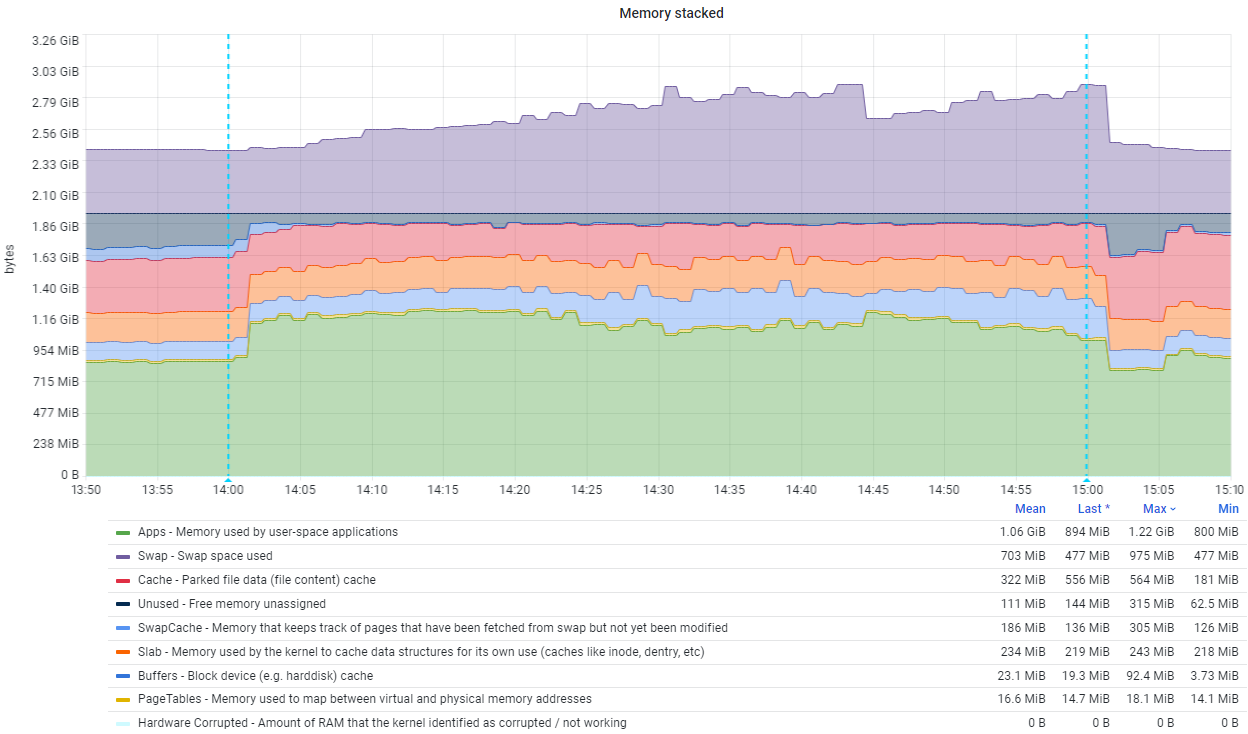
\includegraphics[width=1\textwidth]{img/test_one/memory.png}
    \caption{Wykres skumulowany przedstawiający wykorzystanie dostępnej pamięci przez wirtualną maszynę}
\end{figure}

%\begin{figure}[H]
%    \centering
%    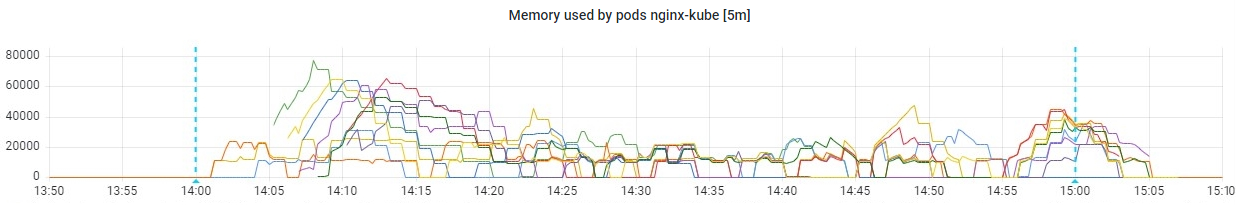
\includegraphics[width=1\textwidth]{img/test_one/memory-pods.png}
%    \caption{Memory pods}
%\end{figure}

Następny wykres prezentuje średnie zużycie rdzeni procesora (w tym przypadku dostępne dla maszyny były dwa rdzenie), przez pody nginx-kube (Rysunek 6.13). Po rozpoczęciu testu serwis obsługiwany był przez trzy pody. Po pięciu minutach wzmożony ruch (około 150 wirtualnych użytkowników) pozwolił utworzyć nowe pody dzięki HPA. 

\begin{figure}[H]
    \centering
    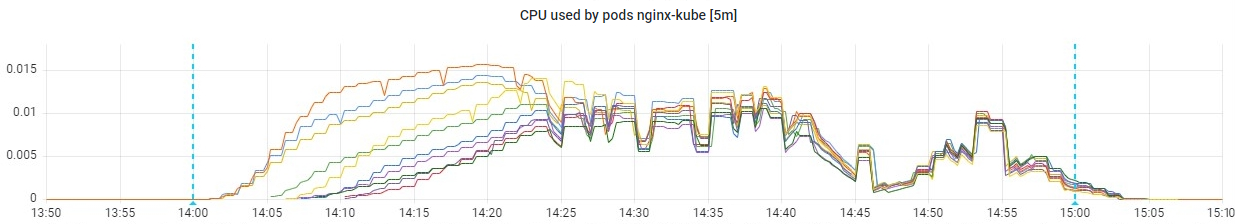
\includegraphics[width=1\textwidth]{img/test_one/cpu-nginx.png}
    \caption{Rdzenie CPU wykorzystywane przez pody nginx-kube, przy czym dostępne były dwa rdzenie}
\end{figure}

Maksymalne zużycie nie przekracza 0,016 rdzenia. Wykres z Rysunku 6.14 również przedstawia wykorzystanie dostępnych rdzeni, tym razem dla wszystkich podów w klastrze. Najbardziej aktywny był pod kube-apiserver-minikube, który jest składową warstwy sterowania.

\begin{figure}[H]
    \centering
    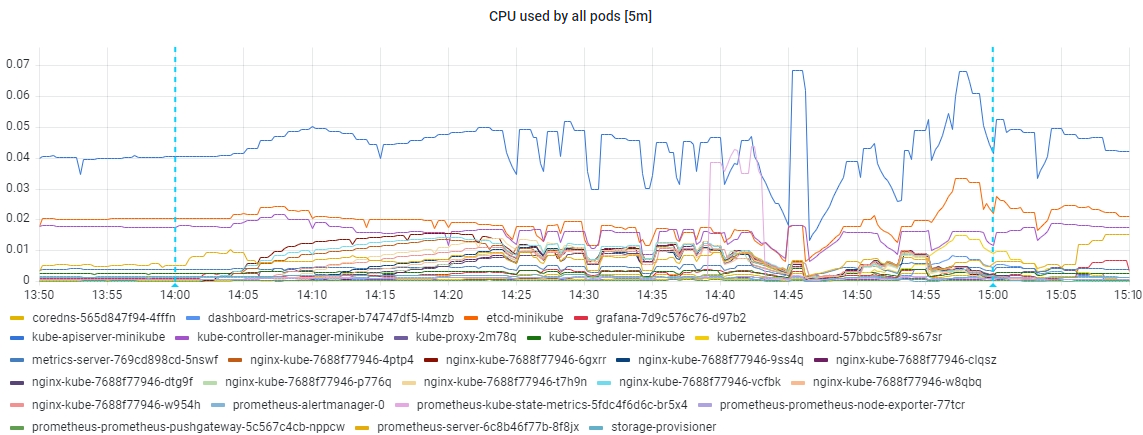
\includegraphics[width=1\textwidth]{img/test_one/cpu-all-pods.png}
    \caption{Rdzenie CPU wykorzystywane przez wszystkie pody w klastrze, przy czym dostępne były dwa rdzenie}
\end{figure}

Następny wykres (Rysunek 6.15) pokazuje procentowe wykorzystanie procesora przez całą maszynę. W pierwszych dwudziestu minutach działania skryptu, gdy inkrementowana jest liczba użytkowników do 600, wzrost użycia stopniowo rośnie. W dalszej części testu skoki w obciążeniu CPU stają się jednak gwałtowne i niejednokrotnie przekraczają 90\%. 

\begin{figure}[H]
    \centering
    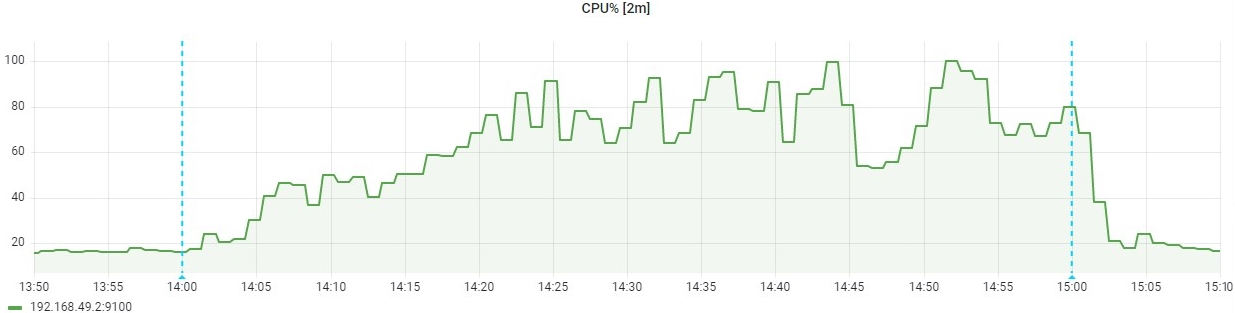
\includegraphics[width=1\textwidth]{img/test_one/cpu-percent.png}
    \caption{Wykorzystanie dostępnego CPU przez maszynę w procentach}
\end{figure}

Newralgicznym momentem jest osiągnięcie 100\% wykorzystania zasobów procesora. Tego rodzaju sytuacja szczególnie wpływa na maszynę, uniemożliwiając płynne działanie całego systemu i spowalniając jego pracę. Stuprocentowe zużycie CPU przez dłuższy czas może prowadzić do przerw w dostawie udostępnianych usług.\\

Skoki w użyciu procesora nie wynikają jednakże wyłącznie z czynników zewnętrznych, takich jak np. ruch sieciowy. Prowadzić do tego mogą również procesy uruchamiane przez samą maszynę lub jej administratora. Drugi test polegał na wykorzystaniu narzędzia Kube-Stresscheck, który wdrażany jest do klastra jako nowy deployment.
\newpage

W celu uruchomienia deploymentu w klastrze Minikube użyto poniższego polecenia:

\scriptbash{files/minikube/commands/stress.txt}

Następnie ww. deployment rozpoczął tworzenie kopii procesu \textit{stress}, który maksymalnie obciąża pamięć i procesor. Po kilku minutach praca systemu została drastycznie spowolniona. Jak można zauważyć na Rysunku 6.16 - średnie obciążenie (ang. \textit{load average}) rosło, a w przeciągu ostatniej minuty 42 procesy oczekiwały na dostęp do zasobów oczekiwały.

\begin{figure}[H]
    \centering
    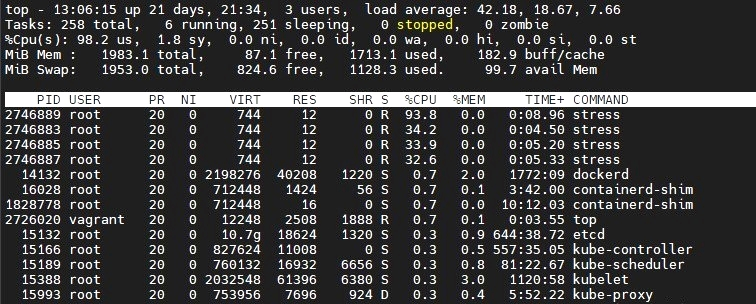
\includegraphics[width=1\textwidth]{img/test_two/top.jpg}
    \caption{Wynik polecenia \textit{top} po kilku minutach od rozpoczęcia testu}
\end{figure}

Klaster Minikube zbudowany jest tylko z jednego węzła, dlatego wszystkie obiekty, również te z warstwy sterowania, są narażone przy tak dużym obciążeniu. Choć Minikube pozostawał aktywny, to jego proces \textit{apiserver} przestawał działać w szczytowych momentach zużycia CPU (Rysunek 6.17). Przekładało się to na ograniczoną możliwość kontrolowania klastra.

\begin{figure}[H]
    \centering
    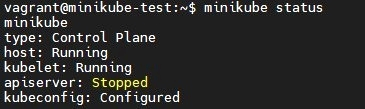
\includegraphics[width=0.5\textwidth]{img/test_two/minikube-status.jpg}
    \caption{Status Minikube i jego procesów}
\end{figure}

Serwer API jest jednym z kluczowych składników warstwy sterowania, który przesyła informacje, a także waliduje oraz konfiguruje dane przeznaczone dla obiektów w klastrze.

Stąd wynikł również problem z użyciem podstawowych poleceń \textit{kubectl} - jeśli \textit{apiserver} posiadał status \textit{Stopped} i nie zdążył być restartowany przez Kubernetesa, wówczas komenda zwracała informację o przekroczeniu czasu na połączenie (Rysunek 6.18).

\begin{figure}[H]
    \centering
    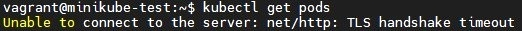
\includegraphics[width=0.7\textwidth]{img/test_two/kubectl-pods.jpg}
    \caption{Przekroczenie maksymalnego czasu oczekiwania na połączenie}
\end{figure}

Test wpłynął również na działanie serwisów w klastrze - zdalny dostęp do platform takich jak Grafana czy Kubernetes Dashboard został uniemożliwiony. W przypadku drugiej z wymienionych platform pojawia się stosowna informacja o problemie z dostępnością serwisu - \textit{Service Unavailable} (Rysunek 6.19).  

\begin{figure}[H]
    \centering
    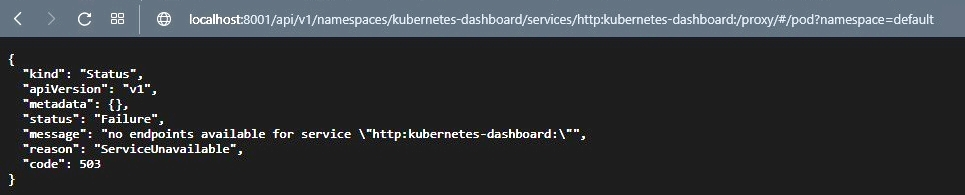
\includegraphics[width=1\textwidth]{img/test_two/dash.jpg}
    \caption{Brak dostępu do Kubernetes Dashboard w trakcie testu}
\end{figure}

Po około czterdziestu minutach z klastra usunięto deployment testu:

\scriptbash{files/minikube/commands/stress_stop.txt}

Następnie w Grafanie sprawdzono dostępne dashboardy oraz oznaczono przybliżone godziny rozpoczęcia i zakończenia testu, kolejno 14:03 oraz 14:49.\\

Na wykresie przedstawiającym procentowe użycie procesora przez wirtualną maszynę (Rysunek 6.20) zauważalne są przedziały czasowe, w których Prometheus nie był w stanie zbierać danych. Jest to związane nie tylko z zatrzymywaniem pracy \textit{apiserver}, ale również podów Prometheusa. 

\begin{figure}[H]
    \centering
    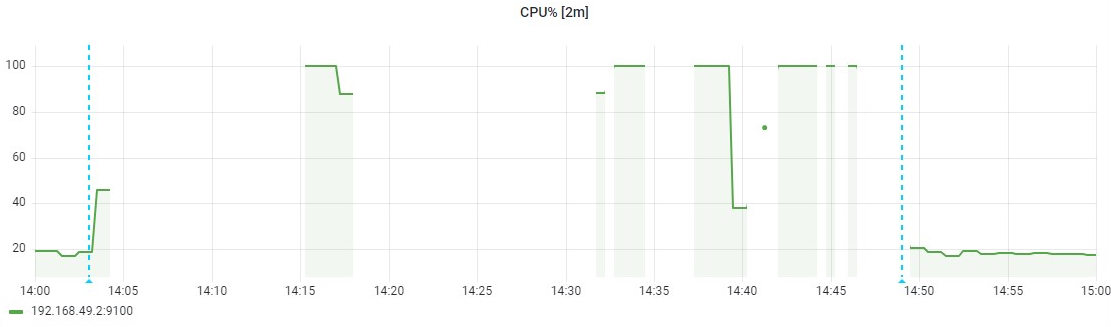
\includegraphics[width=1\textwidth]{img/test_two/cpu.png}
    \caption{Procentowe wykorzystanie dostępnego CPU przez maszynę w trakcie działania testu}
\end{figure}

Po wylistowaniu podów ze wszystkich przestrzeni nazw okazało się, że większość podów obsługujących monitoring było restartowanych w trakcie przeprowadzanego testu (Rysunek 6.21). Podobnie było w przypadku podów z namespace \textit{kube-system}, które to odpowiadają za działanie Kubernetesa.

\begin{figure}[H]
    \centering
    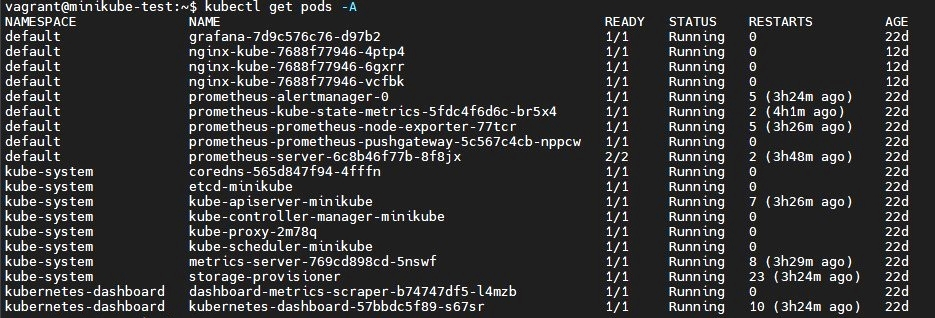
\includegraphics[width=1\textwidth]{img/test_two/pods-all.jpg}
    \caption{Wylistowanie podów ze wszystkich przestrzeni nazw w klastrze}
\end{figure}
\vspace{1em}

Ostatni przeprowadzony test w istotny sposób wpłynął na działanie klastra. Uniemożliwił on dostęp do serwisów, ale co ważniejsze nie pozwalał na płynną administrację klastrem i maszyną. 

W przypadku maszyny wirtualnej doraźnym rozwiązaniem mogłoby być zwiększenie przysługujących jej zasobów, jeśli możliwe jest ich dodanie bez restartu systemu. Należy jednak pamiętać o tym, że komputery i oprogramowanie wymagają przeprowadzania aktualizacji. Stąd klastry jednowęzłowe, choć prostsze w budowie oraz zarządzaniu, nie mogą zapobiec przerwom w dostępności usług. Mogą to zapewnić klastry o większej liczbie węzłów.

Rozproszony system jest w stanie reagować na zmieniające się czynniki dzięki większej liczbie komputerów obsługujących klaster, co pozwala na zminimalizowanie prawdopodobieństwa wystąpienia pełnego \textit{downtime'u}. 


\chapter{Klaster z trzema węzłami}

W celu zbudowania klastra z większą liczbą węzłów należało stworzyć odpowiednio dużo maszyn wirtualnych. Zdecydowano o budowie klastra z jednym węzłem warstwy sterowania (tzw. master) oraz dwoma węzłami roboczymi (znane też jako workery). Schemat infrastruktury przedstawia Rysunek 7.1.\\

W celu przekierowania udostępnionych serwisów wykorzystano otwarte już porty:

\begin{itemize}
    \item 8001 dla Kubernetes Dashboard,
    \item 30001 dla Nginx,
    \item 30002 dla Prometheusa,
    \item 30003 dla Grafany.
\end{itemize}

\begin{figure}[htp]
\makebox[\textwidth][c]{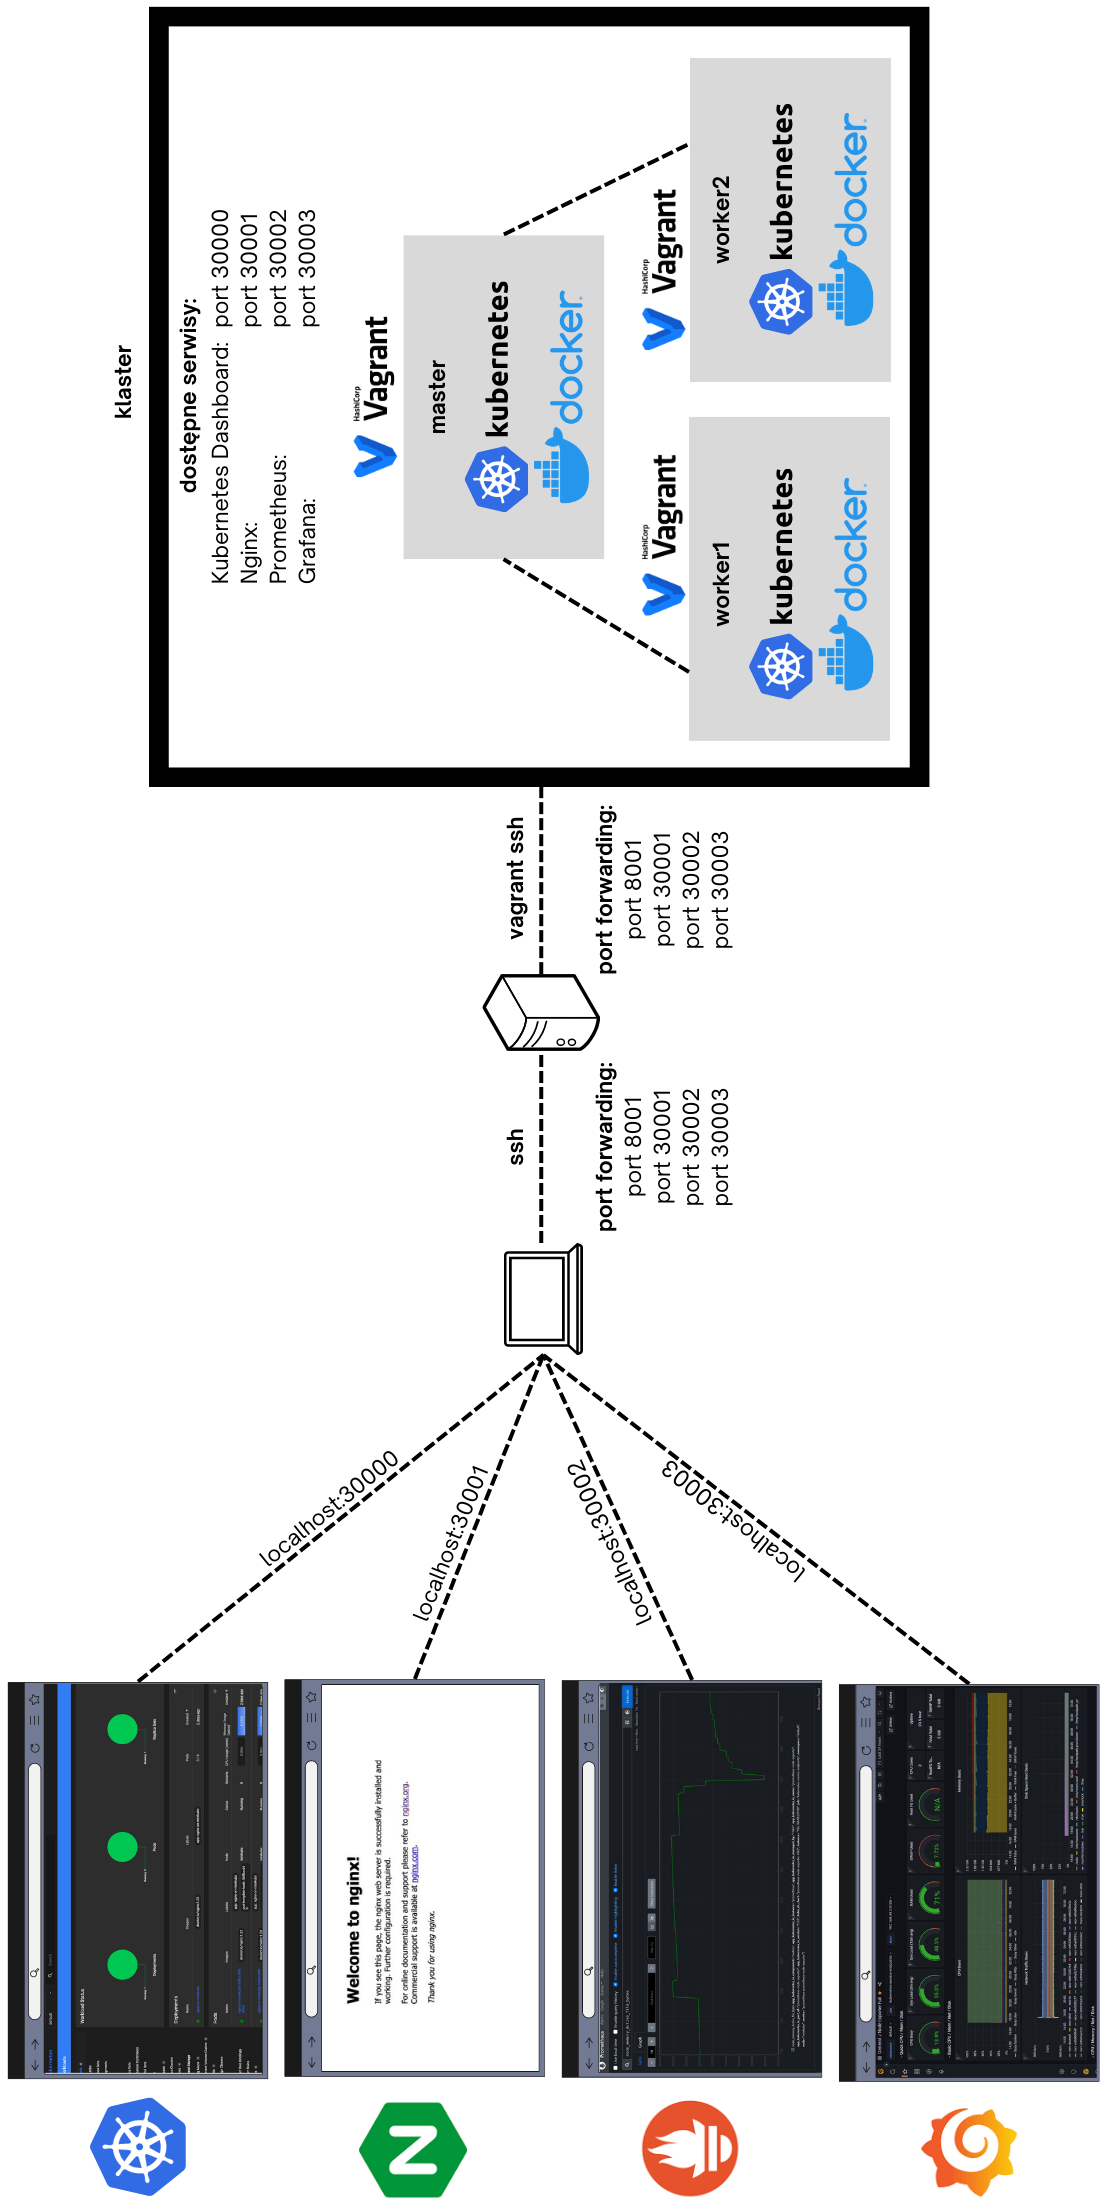
\includegraphics[width=0.85\textwidth]{img2/2nodes.png}}
\caption{Schemat poglądowy infrastruktury dla klastra z trzema węzłami}
\end{figure}
\newpage

Podobnie jak w przypadku klastra z jednym węzłem, do stworzenia maszyn wirtualnych wykorzystano Vagranta z rozszerzeniem \textit{libvirt}. W pliku \textit{Vagrantfile} (Załącznik 9.8) zdefiniowano trzy VM oraz ich parametry. Każda z maszyn wykorzystywała dwa rdzenie pamięci oraz dwa gigabajty pamięci. Otwarto porty dla serwisów wewnątrz klastra, a jako system operacyjny maszyn wirtualnych wykorzystano Ubuntu 20.04 LTS. 

Do budowy klastra użyto MicroK8s - opracowaną przez firmę Canonical lekką dystrybucję Kubernetesa \cite{microk8s}. Za pomocą jednej komendy MikroK8s usprawnia proces instalacji i dokonuje wstępnej konfiguracji maszyn. Na tym etapie każda z maszyn działa jako osobny klaster z własną warstwą sterowania. W celu stworzenia klastra z dwoma węzłami roboczymi, wymagane było zmodyfikowanie wybranej maszyny, aby pełniła rolę mastera. \\

Używając skryptu \textit{get\_nodes\_ip.sh} (Załącznik 9.9), wylistowano adresy IP maszyn oznaczonych jako workery. Adresy te dodano do pliku \textit{hosts} w katalogu \textit{etc} na maszynie mastera w celu zmapowania nazw domenowych z ich adresacją IP, co umożliwi dodanie ich do klastra. Uruchomiona na masterze komenda \textit{microk8s add-node} generuje instrukcję z kodem dla maszyn, które zostaną dołączone do klastra (Rysunek 7.2). Na obu workerach użyto instrukcji z opcją wyłączającą ich warstwę sterowania. Od tego momentu klaster posiada dwa workery oraz jednego mastera (Rysunek 7.3).

\begin{figure}[H]
    \centering
    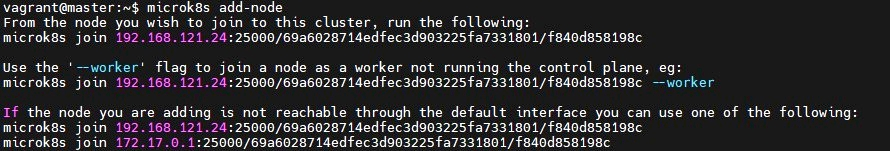
\includegraphics[width=1\textwidth]{img2/addnode1.jpg}
    \caption{Generowanie polecenia dla workerów, umożliwiającego dodanie ich do klastra}
\end{figure}

\begin{figure}[H]
    \centering
    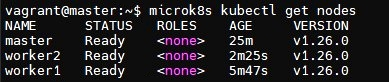
\includegraphics[width=0.5\textwidth]{img2/addnode3.jpg}
    \caption{Wylistowanie węzłów w klastrze za pomocą komendy \textit{microk8s kubectl get nodes}}
\end{figure}

 W trakcie tworzenia maszyn wirtualnych na mastera zostało również ściągnięte repozytorium. Znajdują się tam pliki YAML dla deploymentu i service'u aplikacji Nginx (kolejno Załącznik 5.1 oraz Załącznik 5.2), skrypt służący do testowania wytrzymałości zbudowanej infrastruktury \textit{k6\_test\_cluster.js} (Załącznik 9.7) oraz skrypt konfigurujący \textit{config\_master.sh} (Załącznik 9.10). \\

Skrypt \textit{config\_master.sh} umożliwia zautomatyzowanie konfiguracji klastra i samego mastera. Wyłączana jest możliwość uruchamiania podów aplikacji na węźle warstwy sterowania (Załącznik 9.10, linia 37), dzięki czemu aplikacje obsługiwane będą przez workery. 

%Następnie w skrypcie wywoływana jest komenda, która oznaczy węzeł warstwy sterowania jako mastera. 

W dalszej kolejności instalowane jest narzędzie K6, po czym wdrażana jest aplikacja Nginx wraz z HPA i uruchamiany jest jej serwis. Włączany jest również Kubernetes Dashboard - typ serwisu zmieniono na NodePort i wybrano port 30000 jako domyślny dla Dashboardu. Jako ostatnie wdrażane są Prometheus oraz Grafana - w ten sam sposób, co w przypadku klastra z jednym węzłem. 

Dodatkowo, aby dostać się do serwisów Kubernetes Dashboard, Nginx, Prometheusa czy Grafany spoza sieci klastra, konieczne jest manualne przekierowanie portów - zgodnie z instrukcjami wypisanymi pod koniec pracy skryptu. W przypadku Dashboardu i Grafany wymagane jest również wygenerowanie tokenów dostępu.\\

Po zakończeniu działania skryptu klaster jest przygotowany do dalszej pracy. Po konfiguracji master rozdzielił zadania związane z utrzymaniem aplikacji w klastrze pomiędzy dwa workery (Rysunek 7.4).

\begin{figure}[H]
    \centering
    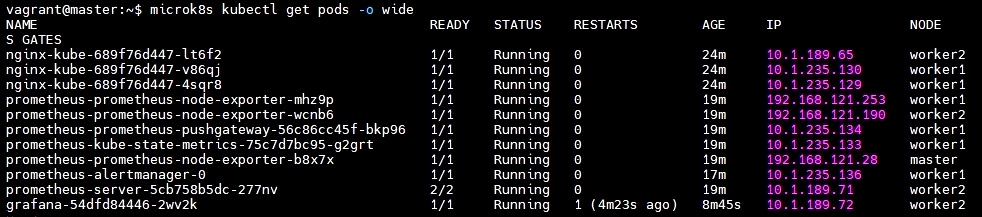
\includegraphics[width=1\textwidth]{img2/apps-wide.jpg}
    \caption{Pody aplikacji działające w namespace default na różnych węzłach}
\end{figure}



\newpage
W celu sprawdzenia stanu węzłów działających w klastrze zastosowano komendę:

\scriptbash{files/microk8s/topnodes.txt}

Rysunek 7.5 przedstawia wynik ww. operacji. Dzięki komendzie możliwe jest sprawdzenie ogólnego stanu węzłów, ich poziom wykorzystania pamięci i CPU. Jak można zauważyć, najwięcej zasobów wykorzystuje węzeł mastera.

\begin{figure}[H]
    \centering
    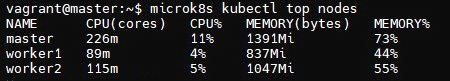
\includegraphics[width=0.7\textwidth]{img2/top-nodes.jpg}
    \caption{Stan węzłów w klastrze}
\end{figure}



\section {Testowanie wydajności klastra z trzema węzłami}

W celu sprawdzenia wydajności stworzonego klastra z dwoma workerami wykorzystano te same narzędzia, co w przypadku testowania klastra z jednym węzłem.

Aby przetestować obciążenie klastra przez napływ użytkowników do udostępnionego serwisu Nginx, wykorzystano ponownie skrypt \textit{k6\_test\_cluster.js} (Załącznik 9.7) oraz oprogramowanie K6. \\

Do analizy wyników wykorzystano Grafanę oraz dashboard Node Exporter Full wraz z dodatkowo zdefiniowanymi panelami dla klastra. Poniższe wykresy przedstawiają przedział czasowy od godziny 16:10 do 17:30, wraz z czasem trwania testu oznaczonym niebieską, przerywaną linią, gdzie test uruchomiony został o godzinie 16:20, a kończy swoje działanie o godzinie 17:20. Przy analizie wyników skupiono się na zużyciu procesora, co było bezpośrednią przyczyną problemów z dostępnością w klastrze jednowęzłowym. \\

Rysunek 7.6 przedstawia średnie zużycie procesora przez pody nginx-kube, które uruchamiane były wyłącznie na węzłach roboczych klastra - sumarycznie dostępne były zatem cztery rdzenie procesora. 

\begin{figure}[H]
    \centering
    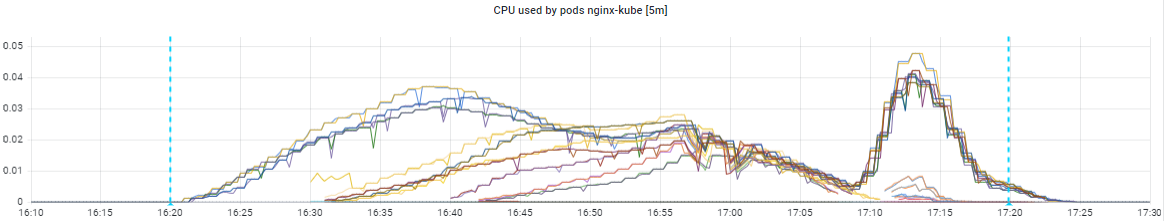
\includegraphics[width=1\textwidth]{img2/test1/cpu_nginx.png}
    \caption{Rdzenie CPU wykorzystywane przez pody nginx-kube - pody te uruchamiane były tylko na workerach, gdzie na każdego z nich przypadały dwa rdzenie procesora}
\end{figure}

Użycie procesora około godziny 17:13, tj. w szczytowym momencie po dostaniu się do serwisu tysiąca użytkowników (linia 11, Załącznik 9.7), osiąga prawie 0,05 rdzenia.

Początkowo serwis nginx-kube obsługiwany był przez trzy pody, lecz wraz ze wzrostem ruchu wirtualnych użytkowników reguła stworzona przez HPA umożliwiła uruchamianie kolejnych podów. Na Rysunku 7.7 zaobserwować można jak węzeł mastera rozdystrybuował siedem nowych podów na workerach.


\begin{figure}[H]
    \centering
    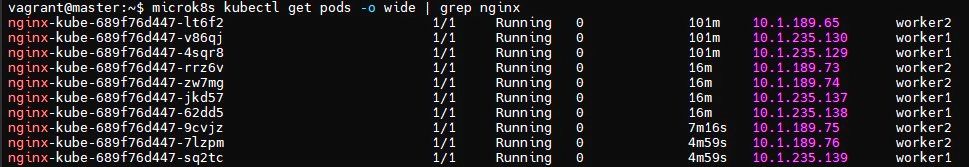
\includegraphics[width=1\textwidth]{img2/test1/nginx.jpg}
    \caption{Dodatkowe pody stworzone dzięki implementacji HPA na maszynie worker1 oraz worker2}
\end{figure}

Wykres z Rysunku 7.8 przedstawia zużycie CPU przez pody ze wszystkich przestrzeni nazw w czasie działania testu. 

\begin{figure}[H]
    \centering
    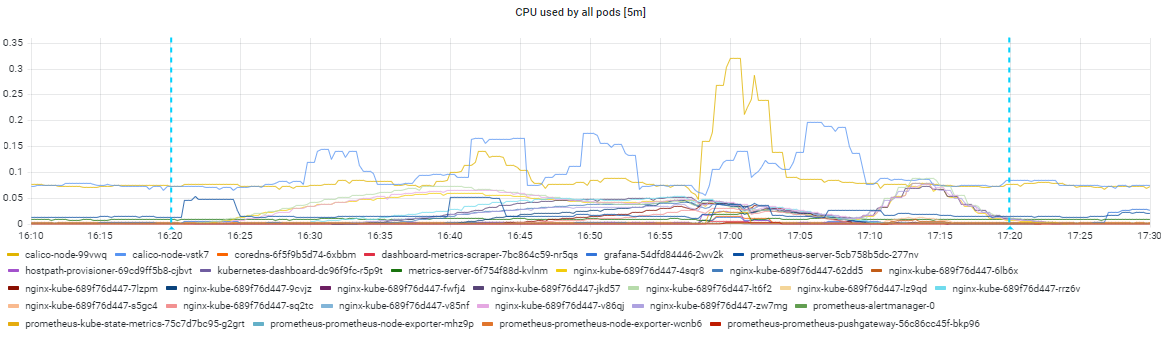
\includegraphics[width=1\textwidth]{img2/test1/cpu_allpods.png}
    \caption{Rdzenie CPU wykorzystywane przez wszystkie pody w klastrze, w tym pody działające na masterze - każda wirtualna maszyna miała dostęp do dwóch rdzeni procesora}
\end{figure}

Największe zużycie, tj. prawie 0,35 rdzenia, obserwowane było w przypadku calico-node. Były to również najbardziej aktywne pody w trakcie trwania godzinnego testu. Calico \cite{calico} to zintegrowany z MicroK8s plugin, ułatwiający konfigurację reguł sieciowych w klastrze oraz umożliwiający masterowi przekierowanie ruchu sieciowego i komunikację z podami węzłów roboczych.

Kolejny wykres (Rysunek 7.9) przedstawia procentowe użycie dostępnych rdzeni procesora przez wszystkie maszyny w klastrze. 

\begin{figure}[H]
    \centering
    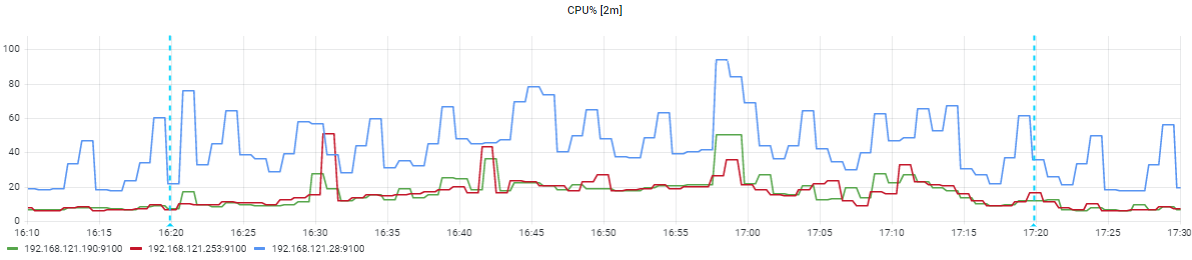
\includegraphics[width=1\textwidth]{img2/test1/cpu.png}
    \caption{Wykorzystanie dostępnego CPU przez wszystkie węzły w procentach}
\end{figure}

Wykorzystanie CPU przez workery oznaczone jest zielonym oraz czerwonym kolorem. Najwyższa osiągana przez nich wartość wynosi około 50\%. Są to jednak chwilowe skoki w zużyciu, ponieważ w trakcie trwania testu zużycie utrzymywało się głównie na poziomie 20 procent.\\

W przypadku mastera, oznaczonego kolorem niebieskim, wartości te są znacznie wyższe. Jako maszyna cyklicznie komunikująca się z workerami i kontrolująca ich zachowanie jest zdecydowanie bardziej obciążona zadaniami, co przekłada się na wzrosty i spadki w wykorzystaniu zasobów. Jeden znaczny skok w zużyciu CPU około godziny 17:57 sięgał ponad 90\%, lecz nie wpłynęło to na działanie samego klastra. Przez cały okres trwania testu infrastruktura pozostawała dostępna, a usługi i działanie serwisów nie było przerwane. \\

Następny test polegał na użyciu Kube-Stresscheck na wybranym węźle roboczym. Celem tego testu było sprawdzenie jak zachowuje się klaster, gdy procesor jednego z workerów zostanie drastycznie obciążony. Test uruchomiono na maszynie worker1, na której działały dwa pody deploymentu nginx-kube, jak i pody związane z działaniem Prometheusa.\\

Po kilku minutach od rozpoczęcia testu sprawdzono stan zużycia pamięci i CPU przez działające w klastrze węzły przy pomocy komendy \textit{microk8s kubectl top nodes}. Na Rysunku 7.10 widoczny jest wynik polecenia. 

\begin{figure}[H]
    \centering
    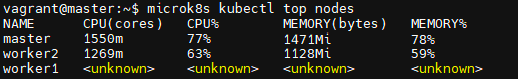
\includegraphics[width=0.7\textwidth]{img2/test2/top.png}
    \caption{Wynik komendy \textit{microk8s kubectl top nodes}}
\end{figure}

Master i worker2 zużywały znacznie więcej zasobów w porównaniu do wcześniejszego użycia ww. komendy, gdy klaster pozostawał w stanie gotowości i żadne dodatkowe akcje nie były podejmowane (Rysunek 7.5). Z kolei stan węzła worker1 pozostawał nieokreślony. 

W celu dalszej diagnostyki użyto komendy \textit{microk8s kubectl get nodes} (Rysunek 7.11) - status węzła worker1 został zmieniony na \textit{NotReady}. Oznacza to, że Kubernetes wykrył na wirtualnej maszynie problem, który uniemożliwia uruchamianie tam podów. 

\begin{figure}[H]
    \centering
    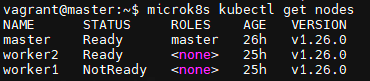
\includegraphics[width=0.5\textwidth]{img2/test2/get-nodes.png}
    \caption{Informacje z węzła roboczego worker1 nie docierają do mastera - maszyna otrzymuje status NotReady}
\end{figure}

Najpopoularniejsze powody tego stanu to m.in. zatrzymanie działania kube-proxy lub kubelet na maszynie, problem z łącznością między danym workerem a węzłem warstwy sterowania itd., lecz w przypadku przeprowadzonego testu wiązało się to z niedostateczną ilością zasobów. Kopie procesu stress przeciążały pamięć i CPU maszyny, uniemożliwiając procesom Kubernetesa prawidłową pracę.\\

Status NotReady wiązał się zatem z wyłączaniem przez Kubernetesa podów na testowanym węźle, które następnie były uruchamiane na maszynie worker2, co obrazuje Rysunek 7.12. 

\begin{figure}[H]
    \centering
    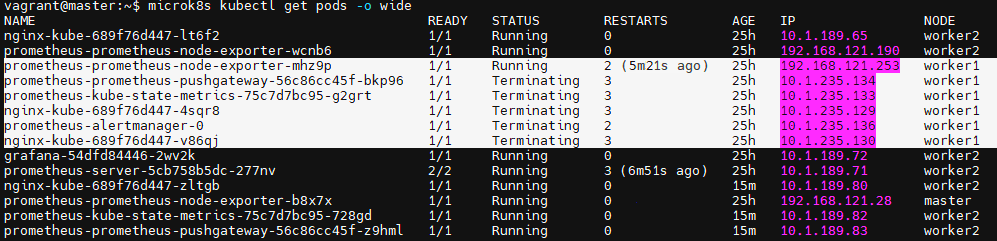
\includegraphics[width=1\textwidth]{img2/test2/pods1.png}
    \caption{Pody na maszynie worker1 zostają wyłączone}
\end{figure}

Na tym etapie wystąpiły problemy z wyświetlaniem danych w Grafanie, ponieważ niektóre z podów Prometheusa musiały zostać wyłączone, a tworzenie nowych zajmowało więcej czasu. Wkrótce po uruchomieniu podów sytuacja się ustabilizowała i aplikacje klastra zaczęły działać ponownie bez wcześniejszych przeszkód.\\

W przypadku serwisu nginx-kube nie zauważono tego typu problemów - pod o nazwie nginx-kube-689f76d447-lt6f2 z drugiego węzła roboczego działał bez żadnych przerw w dostępności w trakcie tworzenia dwóch nowych podów tego deploymentu. Sytuacja ta jednak mogłaby wyglądać zgoła inaczej, jeżeli w trakcie testu wystąpiłoby istotne zwiększenie ruchu sieciowego do serwisu ze strony użytkowników.\\

Tuż po zakończeniu testu ponownie sprawdzono stan podów w klastrze (Rysunek 7.13). Pody z workera1 nadal działały na drugim węźle, jednak łączność z pierwszą maszyną zaczęła być przywracana - zrestartowany został pod, który służy do przesyłania danych z tego węzła do bazy Prometheusa.

\begin{figure}[H]
    \centering
    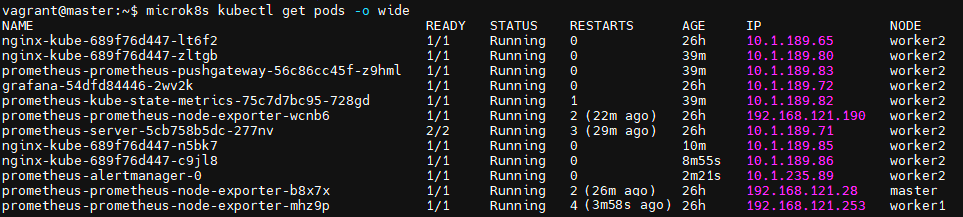
\includegraphics[width=1\textwidth]{img2/test2/pods2.png}
    \caption{Pody działające dotychczas na worker1, uruchomione zostały na węźle worker2}
\end{figure}

Następnie w Grafanie sprawdzono wykres procentowego zużycia procesora w przeciągu jednej godziny (Rysunek 7.14). Pionowe niebieskie linie reprezentują przybliżony czas rozpoczęcia i zakończenia testu, tj. kolejno godzina 16:33 oraz 17:19. 
Czerwonym kolorem oznaczony jest testowany worker1, z kolei niebieski to master, a zielony worker2.

\begin{figure}[H]
    \centering
    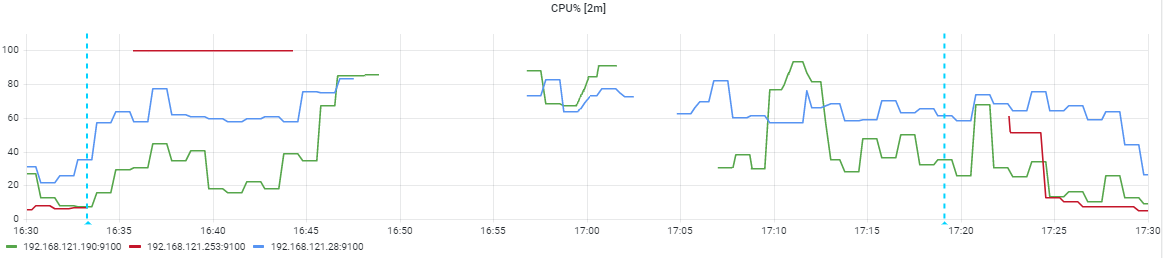
\includegraphics[width=1\textwidth]{img2/test2/cpu-stress.png}
    \caption{Wykorzystanie dostępnego CPU przez węzły w klastrze przedstawione w procentach}
\end{figure}

Przez większą część trwania testu informacje o stanie pierwszego węzła nie docierały do Prometheusa. W początkowej fazie działania testu widoczne jest stuprocentowe wykorzystanie procesora przez workera1. Wówczas zauważalny jest również wzrost zużycia CPU w przypadku mastera i drugiego węzła. \\

Po dziesięciu minutach od rozpoczęcia testu dane ze wszystkich węzłów przestały napływać, co wiązało się z restartami wielu podów, w tym Prometheusa, i ponownym ich uruchamianiem na innej maszynie. 
Można zatem wywnioskować, że przerwy w działaniu jednego z workerów mogą mieć duży wpływ na pracę klastra o małej liczbie węzłów i niewielkiej ilości dostępnych dla nich zasobów. 

W przypadku maszyny worker1 sytuacja nie zmieniała się do końca trwania testu. Jak wspomniano wcześniej, pod przesyłający dane z węzła zaczął działać ponownie dopiero po wyłączeniu oprogramowania testującego. Gdy wykorzystanie CPU spadło wystarczająco, możliwe stało się ponowne nawiązanie komunikacji pomiędzy workerem1 a masterem, przez co nastąpiła zmiana statusu węzła z NotReady na Ready.\\

Ponadto należy zwrócić uwagę na czas, w którym pody są przenoszone po zmianie statusu węzła na NotReady. Domyślnie Kubernetes rozpoczyna proces uruchamiania podów na nowym workerze po pięciu minutach od zmiany ww. statusu. Czas ten można sprawdzić dla konkretnych podów używając \textit{microk8s kubectl describe pod} (Rysunek 7.15). Celem zminimalizowania czasu oczekiwania na przeniesienie podów, wskazana jest zmiana wartości tego parametru.

\begin{figure}[H]
    \centering
    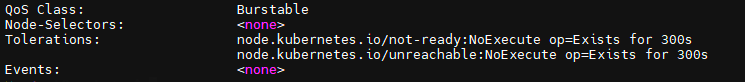
\includegraphics[width=0.9\textwidth]{img2/test2/describe-pod.png}
    \caption{Informacja o zachowaniu jednego z podów nginx-kube podczas sytuacji krytycznej dla działania węzła, na którym się znajduje}
\end{figure}

Głównym problemem w trakcie przeprowadzanego testu były przerwy w dostępności Prometheusa. Pomimo tego klaster utrzymał funkcjonowanie service'u aplikacji Nginx, dzięki wcześniejszemu rozproszeniu podów między dwa workery. Ponadto mimo zwiększonego obciążenia procesora na masterze i drugim węźle, maszyny te przez cały okres trwania testu odpowiadały na komendy bez większych opóźnień.\\

Biorąc pod uwagę wyniki testu, należy podkreślić jak istotne jest dopasowanie odpowiedniej liczby podów deploymentu w infrastrukturze. Rozproszenie podów na węzłach roboczych pozwala utrzymać działanie serwisu, co w przypadku stworzonej infrastruktury umożliwiło dostęp do aplikacji Nginx pomimo \textit{downtime'u} maszyny worker1. 

Ponadto należy zwrócić uwagę na liczbę pracujących w klastrze workerów. Większa ich liczba pozwoliłaby zmniejszyć obciążenie CPU na maszynie worker2. Należałoby rozważyć również dodatkowe maszyny typu master. Tego rodzaju redundancja pomogłaby zabezpieczyć klaster przed nieoczekiwanym zakończeniem działania maszyny węzła warstwy sterowania.




\chapter{Podsumowanie}

Celem pracy było stworzenie dwóch klastrów, z jednym oraz trzema węzłami, a następnie oszacowanie ich wydajności. Do stworzenia maszyn wirtualnych, które miały być hostami w klastrach, użyto narzędzi takich jak oprogramowanie Vagrant, biblioteka \textit{libvirt} oraz natywne dla Linuxa środowisko wirtualizacyjne KVM/QEMU. \\

Do budowy klastra jednowęzłowego wykorzystano Minikube, natomiast w przypadku klastra z wieloma węzłami zastosowano MicroK8s. Dzięki automatyzacji procesu tworzenia maszyn wirtualnych oraz samego klastra za pomocą skryptów powłoki systemowej Bash i narzedzia Helm, wdrażanie infrastruktury nie wymagało nadmiernego nakładu pracy ze strony administratora. Dodatkowo, w klastrze zaimplementowane zostały narzędzia Prometheus oraz Grafana, które służyły do monitoringu stanu maszyn i klastra. \\

W testowaniu wydajności wykorzystano dwa rodzaje testów. Test obciążeniowy przeprowadzony został za pomocą narzędzia K6, z kolei w teście przeciążającym wykorzystano Kube-Stresscheck. Analiza wyników oparta była o wykresy wygenerowane przez narzędzia monitoringu oraz dane pozyskane z klastra.\\

Przeprowadzone testy pozwoliły określić możliwe wąskie gardła (ang. \textit{bottlenecks}). Jeśli chodzi o klaster z jednym węzłem, problemem był brak rozgraniczenia między podami obsługującymi procesy Kubernetesa a podami aplikacji, co w przypadku dużego obciążenia systemu wiązało się z ograniczeniem dostępności nie tylko serwisów, ale też samego systemu operacyjnego maszyny, na której działał klaster. Podobna sytuacja nie miała miejsca w klastrze z dwoma workerami oraz jednym masterem. Na testowanej maszynie część aplikacji była niedostępna do momentu uruchomienia podów na drugim workerze.\\

Ostatecznie wykazano, że klaster złożony z trzech węzłów jest, w przeciwieństwie do jednowęzłowego, o wiele bardziej odporny na przeciążenia oraz \textit{downtime}. Jednakże w specyficznych przypadkach, gdy wymagana jest wysoka dostępność klastra, należy rozważyć wdrożenie większej ilości zarówno maszyn roboczych, jak i maszyn warstwy sterowania.

\chapter{Załączniki}
\scriptruby{files/minikube/Vagrantfile.txt}
\captionof{listing}{Plik \textit{Vagrantfile} dla klastra z jednym węzłem}

\scriptbash{files/minikube/config.txt}
\captionof{listing}{Skrypt \textit{config.sh} wykorzystywany przy konfiguracji klastra z jednym węzłem}

\scriptbash{files/minikube/after_config.txt}
\captionof{listing}{Skrypt \textit{after\_config.sh} wykorzystywany przy konfiguracji klastra z jednym węzłem}

\scriptbash{files/minikube/curl_120s.txt}
\captionof{listing}{Skrypt \textit{curl\_120s.sh}}

\scriptjs{files/minikube/k6_fast_load.txt}
\captionof{listing}{Skrypt \textit{k6\_fast\_load.js}}

\scriptjs{files/minikube/k6_long_load.txt}
\captionof{listing}{Skrypt \textit{k6\_long\_load.js}}

\scriptjs{files/minikube/k6_test_cluster.txt}
\captionof{listing}{Skrypt \textit{k6\_test\_cluster.js}}

\newpage
%\scriptjson{files/minikube/minikube_dashboard.txt}
%\captionof{listing}{Plik JSON - szablon stworzonego dashboardu Grafany}

\scriptruby{files/microk8s/Vagrantfile.txt}
\captionof{listing}{Plik \textit{Vagrantfile} dla klastra z trzema węzłami}
\newpage

\scriptbash{files/microk8s/get_nodes_ip.txt}
\captionof{listing}{Skrypt \textit{get\_nodes\_ip.sh} wykorzystywany przy konfiguracji klastra z trzema węzłami}

\scriptbash{files/microk8s/config_master.txt}
\captionof{listing}{Skrypt \textit{config\_master.sh} wykorzystywany przy konfiguracji mastera w klastrze z trzema węzłami}

\addcontentsline{toc}{chapter}{Bibliografia}
\bibliography{rozdzialX-bibliografia}

%\bibliographystyle{apalike}
\bibliographystyle{unsrt}

\end{document}
